\begin{abstract}
 Assessing the impact of public policies, e.g., affirmative actions for college admission, is crucial to understand the impact of high stake decisions on society but real‐life experiments are complex and can pose ethical challenges hard to overcome. Statistical models and computerized simulations might be valuable tools for circumventing both the complexity and the ethical issues in these contexts. \citeauthor{reardon2018levels} have recently proposed a statistical agent-based model for observing the impact of affirmative actions on college admissions. In this paper, we present the results obtained by trying to re-implement their model and to replicate their results. In a nutshell, while we have been able to replicate the main trends observed in the original paper, the original results and the replicated results diverge slightly, at least partly due to unspecified or inconsistent parameters. The reproduction task has been made harder by the unavailability of the code. Our code is written in Python and fully documented. We make it available online for facilitating additional experiments with this sociotechnical system.
\end{abstract}

\section{Introduction}

The work of \citeauthor{reardon2018levels}~\cite{reardon2018levels} assesses the impact of different college admission policies on the probability of various ethnic groups to be admitted using an agent-based simulation model with parameters ``grounded in real-world''.
Real-life experiments over such sociotechnical systems are complex and costly to setup and run over a long time period (\emph{e.g.}, years) and can in general only be done over limited pilot projects.
By enabling computational experiments over college admission policies, \citeauthor{reardon2018levels} provides a useful environment for researchers focusing on the fairness issues related to the deployment and use of artificial intelligence algorithms.
The proposed model is discussed in great length in the original paper, thus providing a solid basis for understanding it.
However, the code of this simulation model is not publicly available.
In addition, when re-implementing the model, we have faced several issues related to important parts of the model.
First, some values of parameters were missing--e.g., initial colleges' quality--while others were used inconsistently along the paper--such as affirmative actions.
For example, the weight of socioeconomic affirmative action is either applied linearly in accordance with the student's resources or with each decrease of one standard deviation in students' resources.
Second, some parameters described--in natural language--in the paper were actually unused by the model. We tried to guess the appropriate formulas to fit the results and the model description of the original paper.
Nonetheless, we were able to guess their probable values in most cases by trying and comparing our results with those reported in the paper, thus following a trial and error strategy.
Although we did not succeed in replicating all the results, the experiments present similar overall trends.
This paper describes in details our replication attempt.

\section{Model of college admissions}

\citeauthor{reardon2018levels}~\cite{reardon2018levels} proposes an agent-based simulation of the college admission process, mainly based on the model described in previous work~\cite{reardon2016agent}, with the addition of a racial attribute to students and the inclusion of positive discrimination policies.
Note that data of~\cite{reardon2018levels}, \cite{reardon2016agent}, and of our replication is fully simulated.
We provide below a brief overview of the model, referring the interested reader to the original paper for more details. Tables~\ref{tab:const} and~\ref{tab:exp} list the main constants and parameters of the model.

The model consists in two sets of agents: colleges and students.
A new population of 10,000 students is randomly drawn (see Table~\ref{tab:stud}) at each iteration, in which one iteration corresponds to one year.
The 40 colleges are kept for the complete simulation and evolve according to the admissions.

Each iteration is composed of three steps:

\begin{description}

\item[Application step.] Students decide on the ``best'' subset of colleges to apply by taking into account their probability of admission depending on their academic achievement and on each college's quality, with a noisy perception of variables varying with financial resources. That is, \textquote[{\cite{reardon2018levels}}]{high-resources families have better information about college quality}.
To mimic societal biases, both academic achievements and financial resources depend on the race attribute.

\item[Admission step.] Colleges rank applications based on noisy version of academic achievements and accept a number of top students based on the historical acceptance rate. College aim at enrolling 150 students.

\item[Enrollment step.] Students enroll into the best college in which they are admitted.

\end{description}

At the end of each iteration, the colleges' admission rate and quality as well as their probability of admission are updated.

Starting from year 15 (the previous years are used for model
convergence), positive discrimination policies are put in place by a subset of colleges.
More precisely, three type of policies can be introduced:

\begin{description}

\item[Socioeconomic-based affirmative action.] During admission, colleges favor low-income students by increasing their perceived academic achievement.

\item[Race-based recruiting.] During application, students from minority groups favor colleges by increasing their perceived quality, increasing the likelihood of an application.

\item[Race-based affirmative action.] During admission, colleges favor students from minority groups by increasing their perceived academic achievement.

\end{description}

The original experiments are concerned with the impact of using socioeconomic-based (SES) affirmative action combined with race-based recruiting instead of race-based affirmative action. The former two are therefore mostly used together by the colleges.

\begin{figure}[ht]
  \centering
  \begin{tikzpicture}[
    stud/.style={fill=PuOr-K},
    coll/.style={fill=PuOr-E},
    both/.style={diagonal fill={PuOr-K}{PuOr-E}},
    iter/.style={->, dashed},
    ]
    \node[stud] (Race) {Race};
    \node[right=of Race, stud, align=center] (Ach) {Achievement,\\ Resources};
    \node[below=of Ach, coll] (Qual) {Quality};
    \node[right=of Ach, both] (PAdmit) {P(Admission)};
    \node[right=of PAdmit, both] (Apply) {Applications};
    \node[below=of Apply, both] (Admit) {Admissions};
    \node[below=of Admit, both] (Enroll) {Enrollment};
    \node[fit=(Apply)(Admit)(Enroll), draw, opacity=.5] (AppAdmEnr) {};
    \draw[->] (Race) -- (Ach);
    \draw[->] (Ach) -- (PAdmit);
    \draw[->] (Qual) -- (PAdmit);
    \draw[->] (PAdmit) -- (Apply);
    \draw[->] (Apply) -- (Admit);
    \draw[->] (Admit) -- (Enroll);
    \draw[->] (Qual) -- (AppAdmEnr);
    \draw[->] (Ach) to[bend left] (AppAdmEnr.100);
    \draw[iter] (Admit) -- (PAdmit);
    \draw[iter] (Ach) -- (Qual);
    \draw[iter] (Enroll) -- (Qual);
    \draw[iter] (Qual) to [out=180,in=270,loop,looseness=4.8] (Qual);
  \end{tikzpicture}
  \caption{Simplified causal model of~\cite{reardon2018levels} with most of the variables being abstracted away.
Students' variables are \colorbox{PuOr-K}{orange}, colleges' variables are \colorbox{PuOr-E}{purple}, while final variables defined for pairs of student and college have both colors.
Dashed arrows represent dependency over past iterations.}
  \label{fig:model}
\end{figure}

\begin{table}[!ht]
    \centering
    \begin{tabular}{l r r r r} \toprule
        \textbf{Race} & \textbf{Weight} & \textbf{Achievement} & \textbf{Resources} & \textbf{corr(Ach, Res)} \\ \midrule
        Asian & 5\% & $\mathcal{N}(1038, 202^2)$ & $\mathcal{N}(0.012, 0.833^2)$ & 0.441 \\
        Black & 15\% & $\mathcal{N}(869, 169^2)$ & $\mathcal{N}(-0.224, 0.666^2)$ & 0.305 \\
        Hispanic & 20\% & $\mathcal{N}(895, 185^2)$ & $\mathcal{N}(-0.447, 0.691^2)$ & 0.373 \\
        White & 60\% & $\mathcal{N}(1052, 186^2)$ & $\mathcal{N}(0.198, 0.657^2)$ & 0.395 \\ \bottomrule
    \end{tabular}
    \caption{Student population}
    \label{tab:stud}
\end{table}

\begin{table}[!ht]
    \centering
    \begin{tabular}{l r} \toprule
        \textbf{Description} & \textbf{Value} \\ \midrule
        %
        Number of colleges & 40 \\
        Number of students & 10000 \\

        %
        College capacity & 150 students / college \\
        %
        Expected yield window & \emph{up to} 3 years (after first year) \\
        Admission probability window & 5 years (after 5\textsuperscript{th} year) \\
        Introduction of policies & 15\textsuperscript{th} year \\ \bottomrule
    \end{tabular}
    \caption{Fixed model parameters}
    \label{tab:const}
\end{table}


\section{Method}

We have mostly followed the detailed description of the model given in~\cite[Appendix~C]{reardon2018levels}.
We have also referred to~\cite{reardon2016agent}, which is often cited by the authors as an inspiration for this work.
Code for this latter model is available in the (proprietary) Stata programming language~\cite{reardon2016stata}.
We have read this code for clarification but we were not able to run it\footnote{Executing this model seems to require Stata version 11, but the dependency ``\texttt{college sorting napps.do}'' is not distributed in the archive.}.
We have contacted the first two authors of~\cite{reardon2018levels} (Sean F. Reardon and Rachel Baker) in May 2021 but got no answer as of May 2022.

For our implementation, we have used the Python programming language, with most of the processing done using \href{https://numpy.org/}{NumPy}.
We use \href{https://scikit-learn.org/}{scikit-learn} for the logistic regression%
\footnote{We also also used \href{https://www.statsmodels.org/}{statsmodels} during development however its interface was less suitable to a pre-parametrized model, which we require for the first 5 iterations.}.

We have experimented with the \href{https://xarray.dev/}{Xarray} library, which provides labeled multidimensional arrays.
Our motivation was to deduplicate the join between students and colleges.
However, we have achieved no storage or time improvement by doing so.

In addition to the replication effort, we focused on execution speed to be able to use the model as a synthetic data generator in other works. For this purpose, random data for all future iterations is drawn at initialization.

\section{Difficulties}\label{sec:diff}

In this section, we present the main issues encountered with respect to the description of the model in the original paper~\cite{reardon2018levels}.
Hereafter, inconsistent descriptions are quoted but we refer the reader to the full paper for more context.
Afterwards, we describe the interpretation that we have followed for the results presented in this paper.

\paragraph{Socioeconomic status (SES)-based affirmative action.}

\begin{itemize}

\item\textquote[{\cite[Section~3]{reardon2018levels}}]{It is during the calculation of $A^{**}_{cs}$ that colleges with an affirmative action policy apply additional weight to a student's perceived admissions desirability in accordance with that policy.
This additional weight is captured by the term $T_c \times [G \times (Black_s \mid Hispanic_s ) + H \times resources_s ]$.
In this term, $T_c$ indicates whether a college has an affirmative action policy, \textelp{} $H$ is the size of the weight given to students under SES-based affirmative action
policies, which is applied \emph{linearly in accordance with the student's resources}, $resources_s$.}

\item\textquote[{\cite[Section~4]{reardon2018levels}}]{SES-affirmative action (corresponding to an increase in admissions consideration of 0, 50, 100 and 150 \emph{achievement points for each decrease of one standard deviation} in applicants' resources);}.

\end{itemize}

Using $H \times resources_s$ as in the first quote would advantage high-income students, which is the opposite of the objective. Moreover, the weight would not follow the description of the next two quotes, which involve the standard deviation. In our implementation, a weight $H \times \max(-\mathrm{zscore}({resources}_s), 0)$ is added to the score of low-income students students, with $\mathrm{zscore}$ being the standard score\footnote{The zscore variable is the number of standard deviations by which the value of a raw score is above or below the mean value of what is being observed or measured} with respect to $resources$, and $H$ the size of the weight (\emph{e.g.}, 0, 50, 100 and 150).
We keep only negative values of the standard score (see Figure~\ref{fig:c4_pen} for a version without truncation) to impact only low-income students (``for each decrease of one standard
deviation'').
Note that our interpretation is not totally satisfactory (see Section~\ref{sec:results}), however we had no success either with the formula of the first quote (see Figure~\ref{fig:c4_f1}).

\paragraph{Quality and own achievement reliability.}

\begin{itemize}

\item\textquote[{\cite[Table~1]{reardon2018levels}}]{Quality reliability and own achievement reliability \emph{bounded by minimum values of 0.5 and maximum values of 0.9.}}

\item\textquote[{\cite[Appendix~C]{reardon2018levels}}]{the reliability of student perceptions of their own achievement, is a function of student resources and \emph{bounded between 0.5 and 0.9}}

\item\textquote[{\cite[Appendix~C]{reardon2018levels}}]{the reliability of student perceptions of college quality, is a function of student resources and \emph{bounded between 0.5 and 0.7}}

\end{itemize}

We assume that 0.7 is a typo and clip the values between 0.5 and 0.9. The impact is however quite negligible (compare  Figures~\ref{fig:c4} and~\ref{fig:c4_pq07}).

\paragraph{Race-targeted recruiting.}

\textquote[{\cite[Appendix~C]{reardon2018levels}}]{Colleges' binary recruitment statuses ($S_c$)---which had previously all been 0---are set based on model parameters that determine which colleges will use recruitment \textelp{}
Utility is then calculated using model-specific recruitment magnitude values ($L$): $ U^*_{cs} = a_s + b_s \times Q^*_{cs} + R_{sc} $. }

There is no use of $S_c$ in the document apart from the definition, and $R_{sc}$ is also not defined.
We assume that it is a typo and that $S_c$ is to be understood as $R_{sc}$.
The recruitment magnitude value $L$ is not used (but is an experimental parameter later).
No specific definition of race-targeted recruitment is given but from \blockquote[{\cite[Section~3]{reardon2018levels}}]{Recruitment efforts work in part by making students aware of specific colleges and by making these colleges seem more appealing to prospective students through additional, targeted contact with those students.} our understanding is that targeted groups have an increased chance of applying to colleges using race-targeted recruitment.
However, the race attribute is not used in conjunction with $L$.

We assume that the race-targeted recruitment weight is added to the perceived utility of attending colleges for minority students, such that \[ U^*_{cs} = a_s + b_s \times Q^*_{cs} + R \times (Black_s \mid Hispanic_s ) \times {T'}_c \] in which ${T'}_c$ indicates whether a college uses race-targeted recruitment and $R$ is the recruitment weight.

\paragraph{Quality update window.}

It is unclear whether the quality of colleges depends only on the previous year or on the past five years:

\begin{itemize}

\item\textquote[{\cite[Appendix~C]{reardon2018levels}}]{Colleges' quality values ($Q_c$) are \emph{updated based on the incoming class of enrolled students before the next year's cohort} of students begins the application process}.

\item\textquote[{\cite[Figure~C5]{reardon2018levels}}]{College quality is \emph{calculated as the five-year running average} of enrolled student caliber.}

\end{itemize}

The later point is given in the caption of a figure, whereas the first is part of the model description.
Using only the previous year to update colleges' quality gives satisfying results (see Figure~\ref{fig:c5}).
Thus, we assume that the five-year running average is not used for the model but only to smooth the plots.

\paragraph{Initial college quality.}

\textquote[{\cite[Appendix~C]{reardon2018levels}}]{Initial college quality ($Q$) is normally distributed}, but the values of the mean and variance are not given.
We relied on the values from~\cite{reardon2016agent}: $Q \sim \mathcal{N}(1070, 130^2)$.

\paragraph{Admission probability estimation.}

After the fifth iteration, each iteration requires fitting a logistic model on submitted application over the past five years. This allows students to estimate their probability of admission into each colleges, which is required for them to select a subset to apply to.

Apart from a significant speed increase, we observe no difference when fitting on the previous year only (and using the previously fitted model's parameters to initialize the new fit).
However, our code still uses the past five years.

\paragraph{Weights of affirmative actions and targeted recruitment.}

\textquote[{\cite[Figure~C3]{reardon2018levels}}]{\emph{moderate} SES-based affirmative action and moderate race-based recruitment, which corresponds to a weight of 100 and 75, respectively.}

\textquote[{\cite[Figure~C3]{reardon2018levels}}]{\emph{strong} SES-based affirmative action and strong race-based recruitment, which corresponds to a weight of 100 and 75, respectively.}

\section{Experiments}

Figures~\ref{fig:c1} to~\ref{fig:A5} present side by side examples of reproduction, with plots taken from the preprint version~\cite{reardon2018levels_preprint} of the original paper~\cite{reardon2018levels} (due to copyright issues) along with our replication results. %
We attempt to replicate a representative subset of the plots, covering the gist of the model: impact of race-based affirmative action (Figures~\ref{fig:c2}, \ref{fig:A4}, \ref{fig:A5}) and impact of SES-based affirmative action and race-based recruitment (Figures~\ref{fig:c4} to~\ref{fig:A3}). %
Additional replications are available in Appendix~\ref{sec:add}.
Table~\ref{tab:exp} describes the available parameters and the values used in the experiments.

Figures~\ref{fig:A2} to~\ref{fig:A5} present the impact of the different strategies on the final (years 25 to 29) composition--racial and socioeconomic\footnote{Our socioeconomic distribution is represented by the quintiles of the \emph{full} students' resources distribution (not only the enrolled students) as doing otherwise results in incomparable categories.}--of enrolled students in colleges. %
Our replication effort involved experimenting with the full set of plots presented in the original paper.
We also resorted to additional plots (not presented in the original paper or the current one) to assess the correlation between admission probability and academic achievement.
Every experiment results from an average of 10 runs.

\begin{table}[!ht]
    \centering
    \begin{tabular}{l r} \toprule
        \textbf{Description} & \textbf{Domain} \\ \midrule
        %
        Number of years & 30, 50 \\
        Number of top colleges implementing policy & 0, 4 \\
        Race-based affirmative action weight & 0, 150, 300, 260 \\
        SES-based affirmative action weight & 0, 50, 75, 100, 150 \\
        Race-based recruiting weight & 0, 25, 50, 100 \\ \bottomrule
    \end{tabular}
    \caption{Experimental parameters}
    \label{tab:exp}
\end{table}


\begin{figure}[p]
  \centering
  \subfloat[{Original (reprinted from~\cite[Figure~C1]{reardon2018levels_preprint})}]{{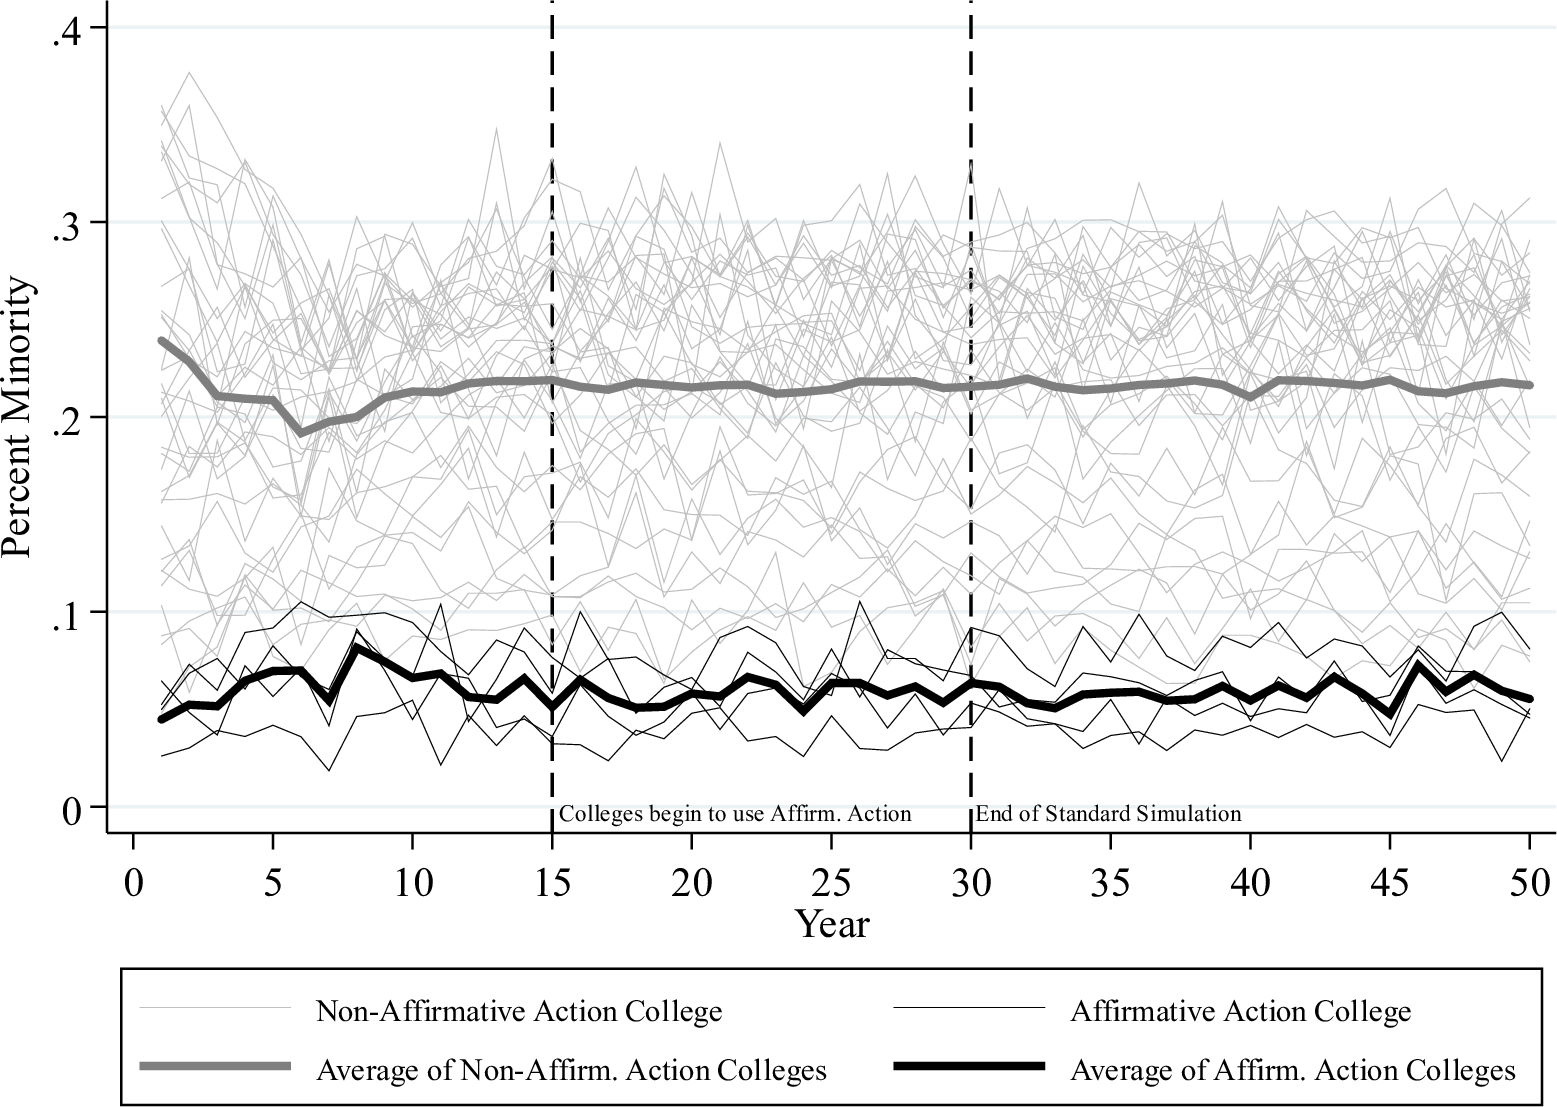
\includegraphics[width=.49\textwidth]{figures_original/figC1.png}}}%
  \hfill%
  \subfloat[{Replication}]{%
    \raisebox{6mm}[0pt][0pt]{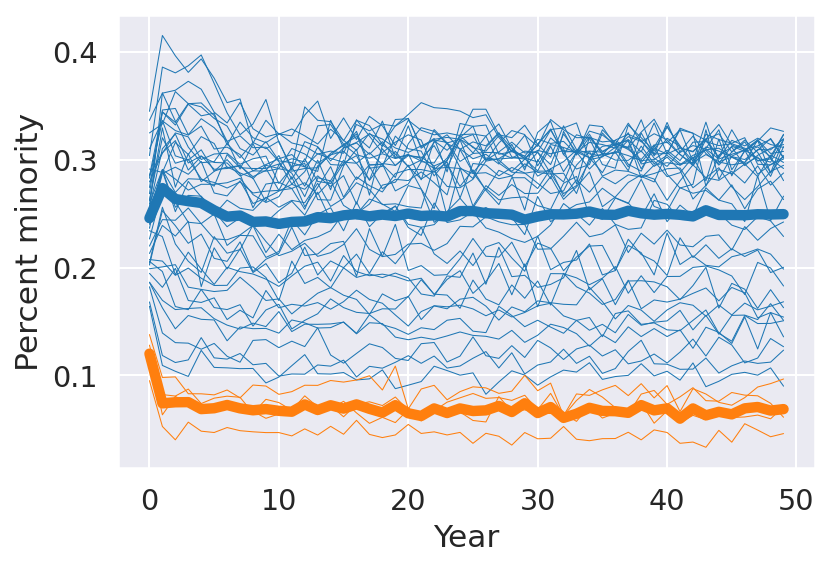
\includegraphics[width=.4\textwidth]{figures/figC1.png}}
  }%
  \caption{Minority enrollment without using affirmative action or recruiting.}
  \label{fig:c1}
\end{figure}

\begin{figure}[p]
  \centering
  \subfloat[{Original (reprinted from~\cite[Figure~C2]{reardon2018levels_preprint})}]{{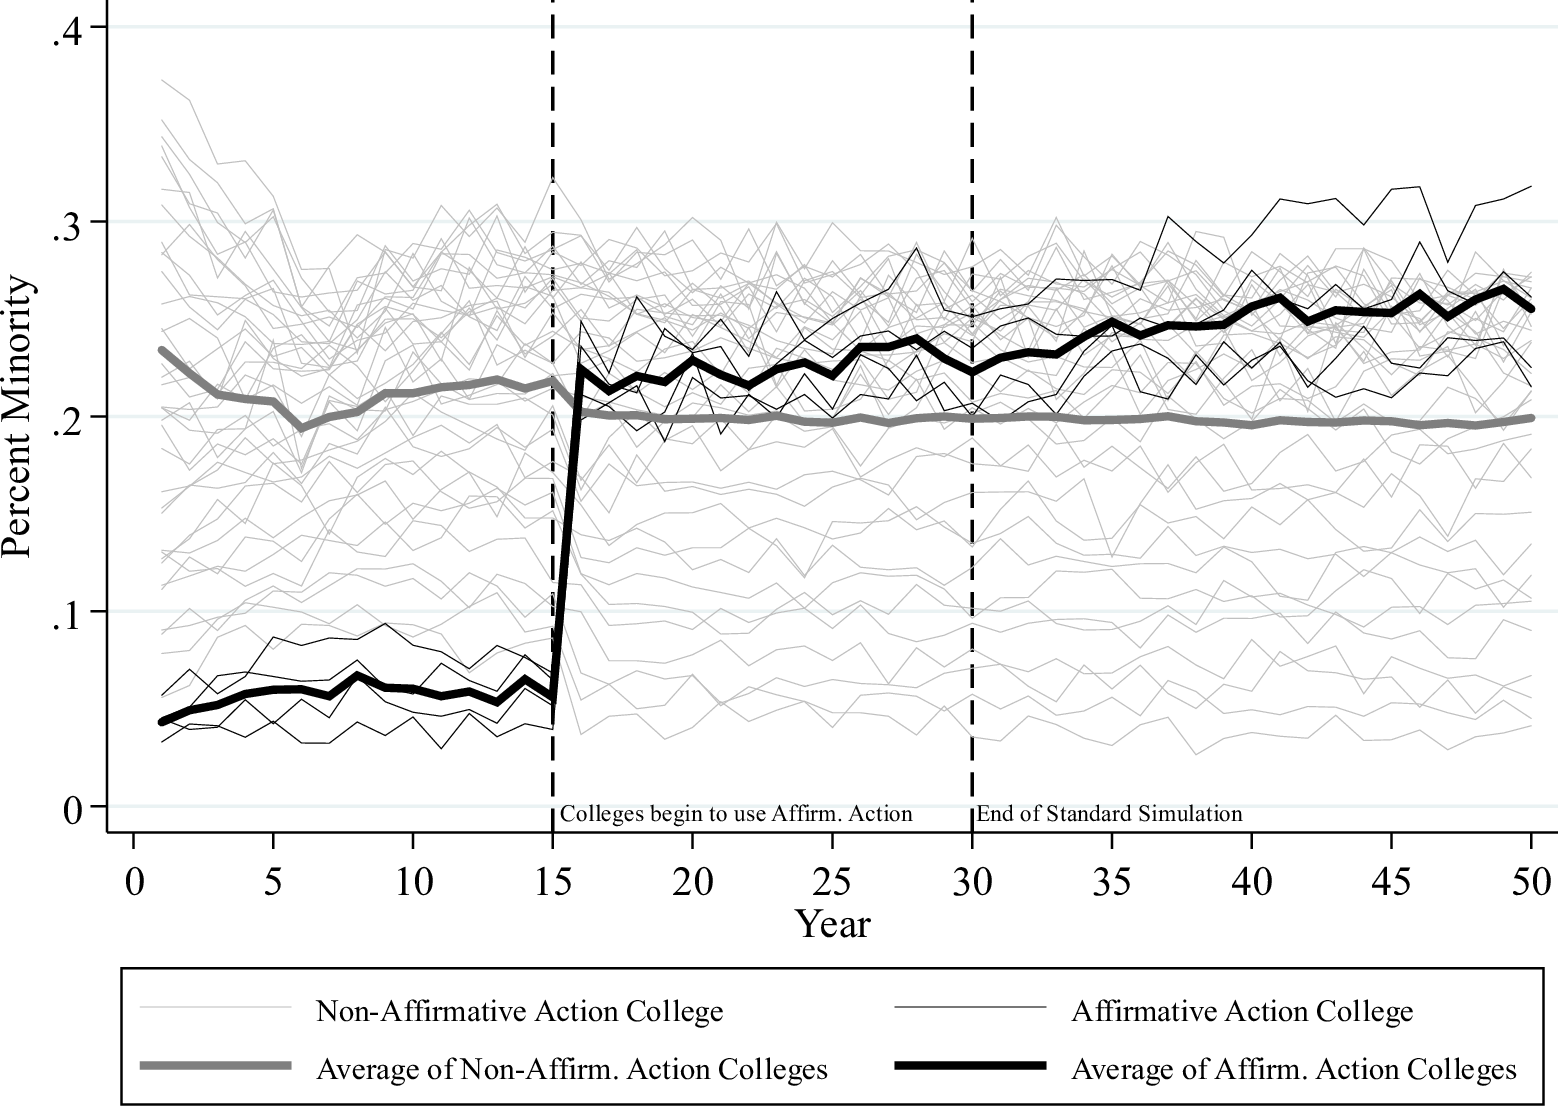
\includegraphics[width=.49\textwidth]{figures_original/figC2.png}}}%
  \hfill%
  \subfloat[{Replication}]{{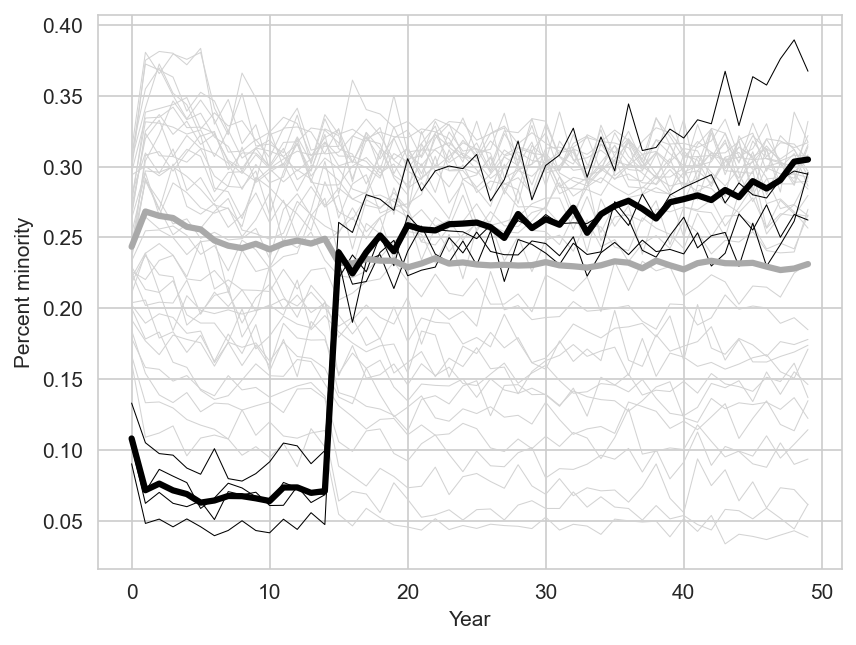
\includegraphics[width=.49\textwidth]{figures/figC2.png}}}%
  \caption{Minority enrollment with the top four colleges using real-world race-based affirmative action (weight of 260).}
  \label{fig:c2}
\end{figure}

\begin{figure}[p]
  \centering
  \subfloat[{Original (reprinted from~\cite[Figure~C4]{reardon2018levels_preprint})}]{{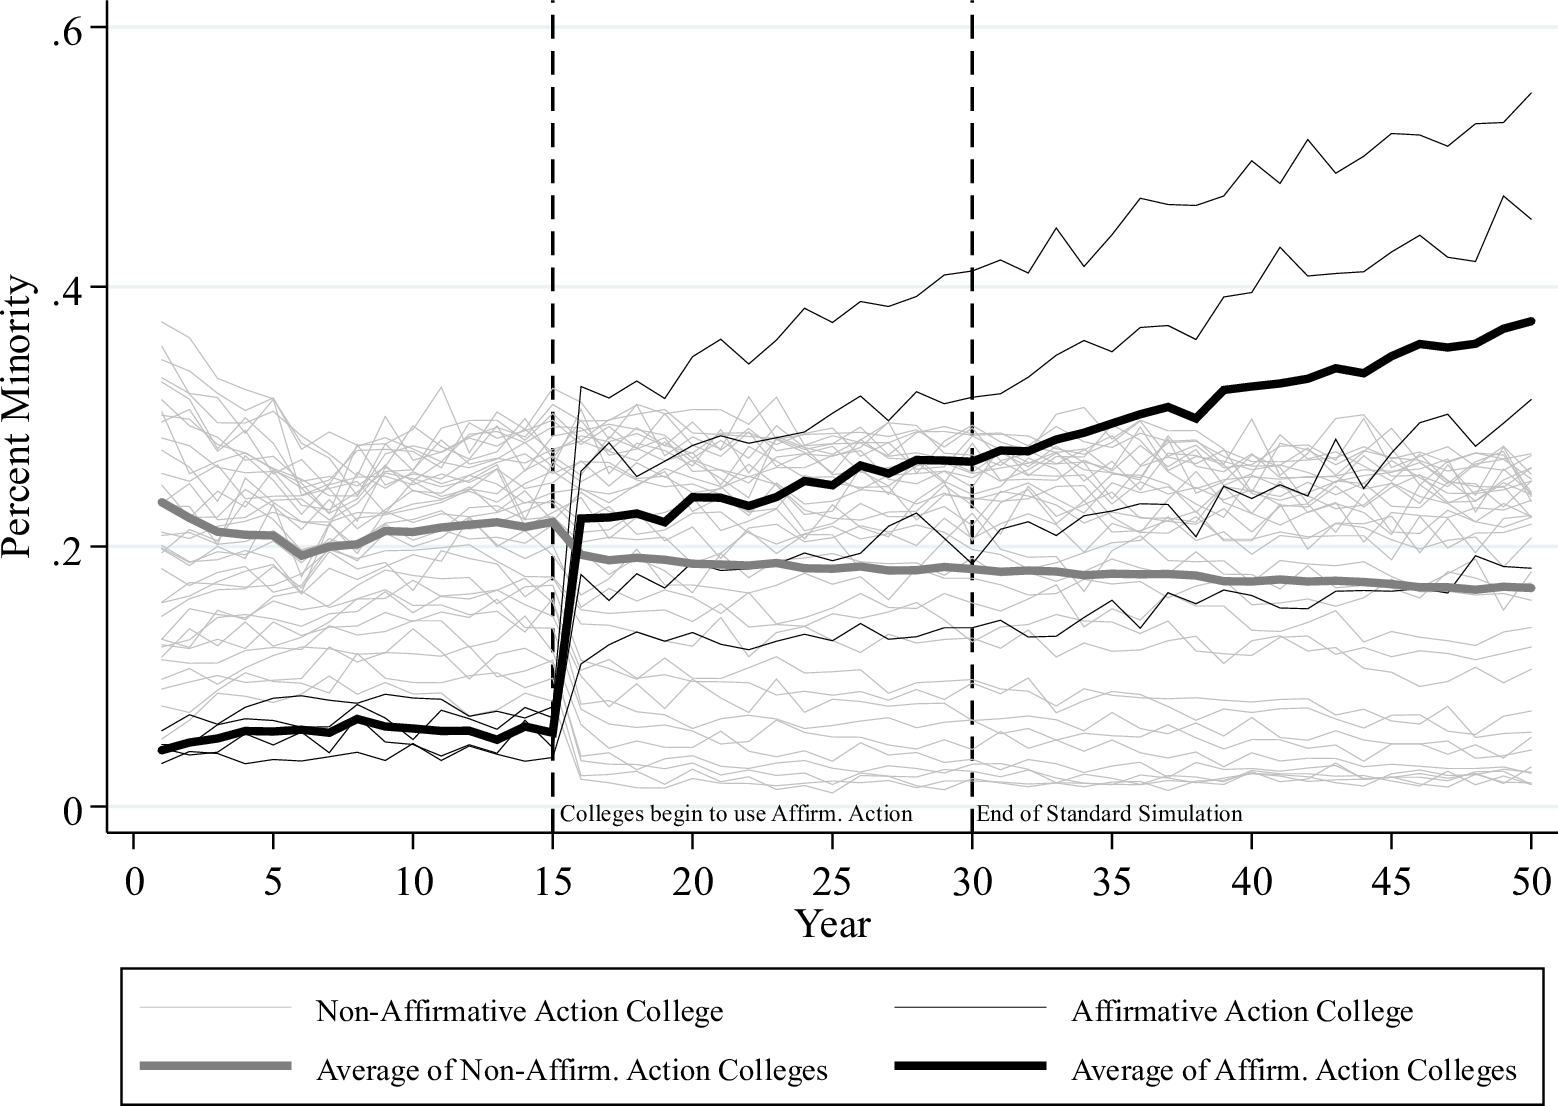
\includegraphics[width=.49\textwidth]{figures_original/figC4.png}}}%
  \hfill%
  \subfloat[{Replication}]{{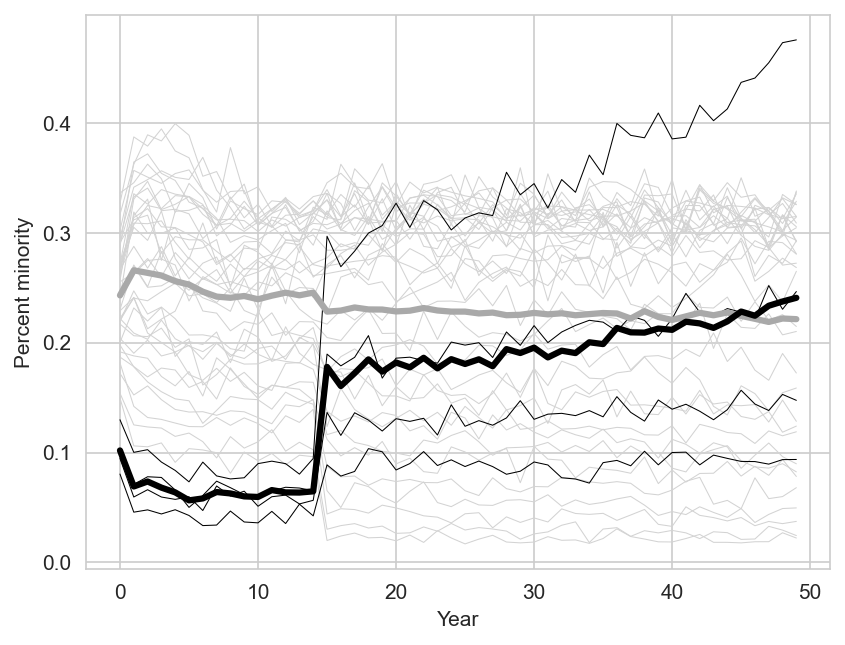
\includegraphics[width=.49\textwidth]{figures/figC4.png}}}%
  \caption{Minority enrollment with the top four colleges using strong SES-based affirmative action (weight of 150) and strong race-based recruitment (weight of 100).}
  \label{fig:c4}
\end{figure}

\begin{figure}[p]
  \centering
  \subfloat[{Original (reprinted from~\cite[Figure~C5]{reardon2018levels_preprint})}]{{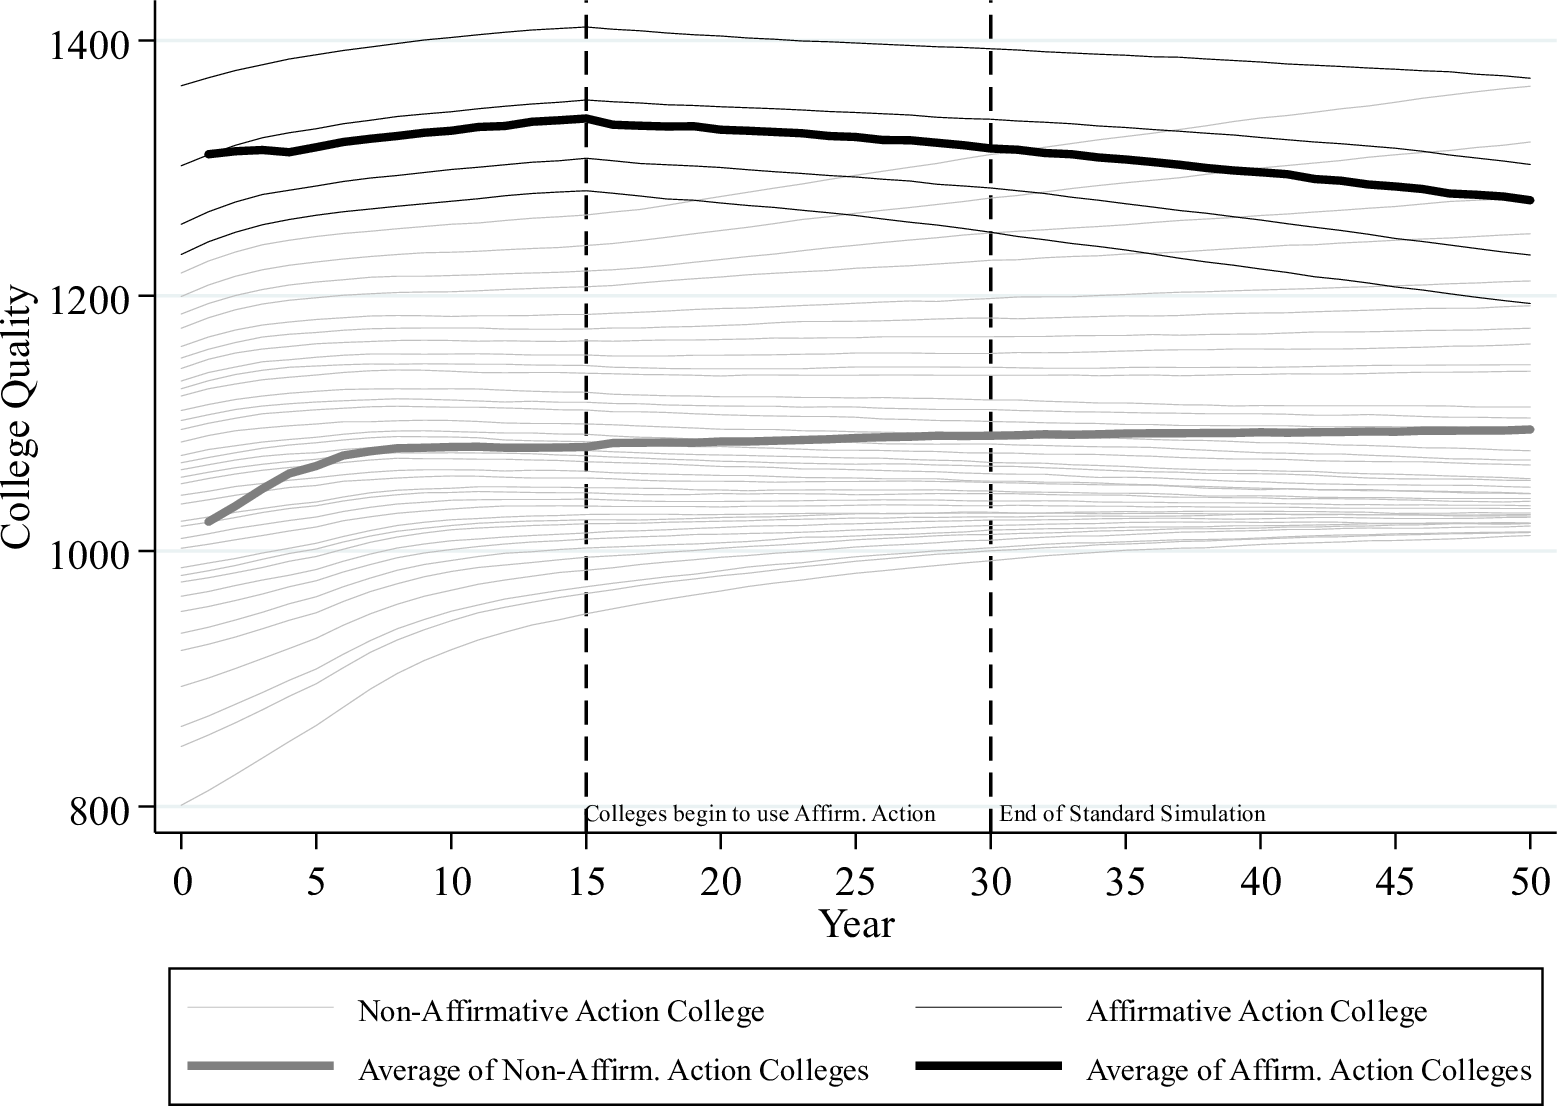
\includegraphics[width=.49\textwidth]{figures_original/figC5.png}}}%
  \hfill%
  \subfloat[{Replication}]{{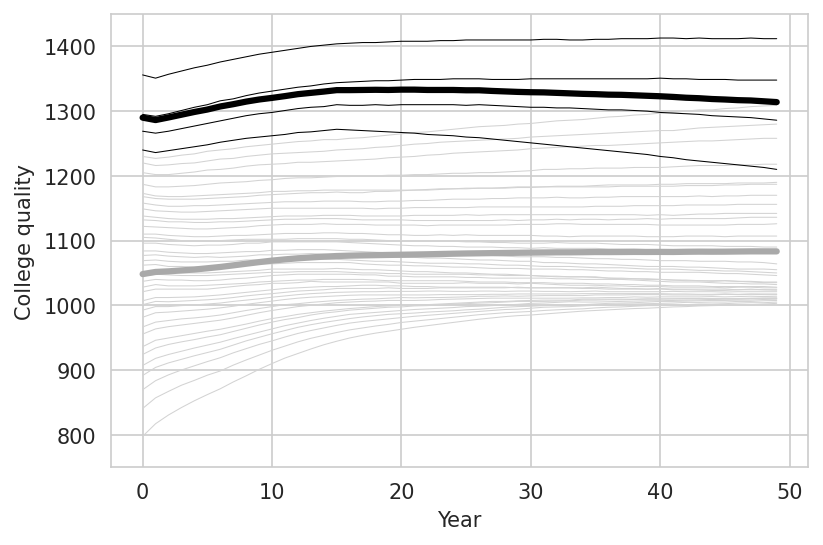
\includegraphics[width=.49\textwidth]{figures/figC5.png}}}%
  \caption{College quality with the top four colleges using strong SES-based affirmative action (weight of 150) and strong race-based recruitment (weight of 100).}
  \label{fig:c5}
\end{figure}

\begin{figure}[p]
  \centering
  \subfloat[{Original (reprinted from~\cite[Figure~D1]{reardon2018levels_preprint})}]{{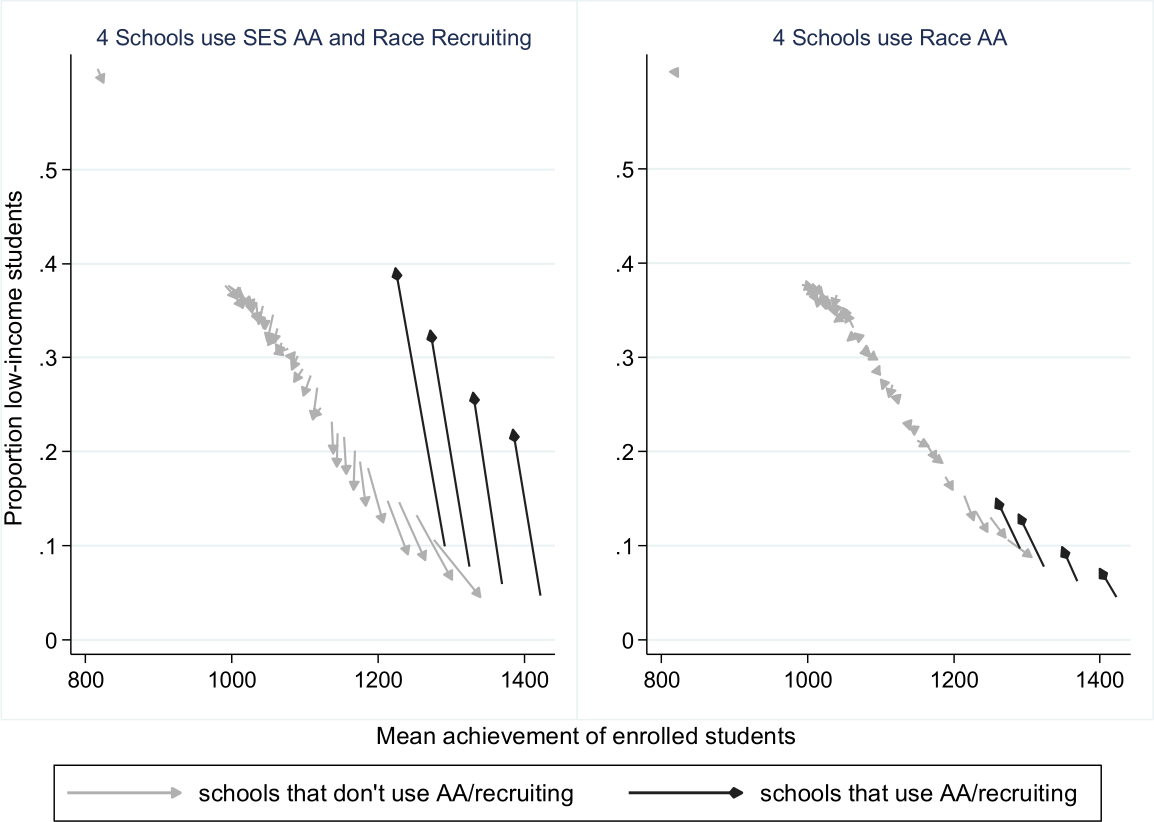
\includegraphics[width=.48\textwidth]{figures_original/figD1.png}}}%
  \hfill%
  \subfloat[{Replication}]{{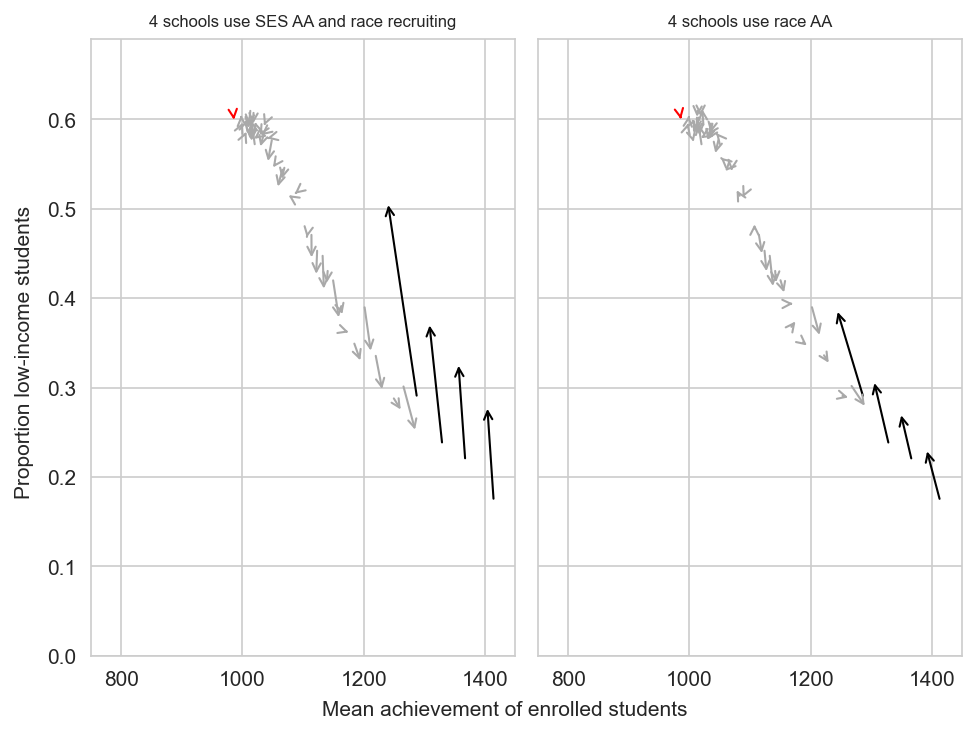
\includegraphics[width=.51\textwidth]{figures/figD1.png}}}%
  \caption{Mean achievement and proportion low-income with top four colleges using (respectively not using) strong SES-based affirmative action (weight of 150) and strong race-based recruitment (weight of 100) on the left sides, and real-world race-based affirmative action (weight of 260) on the right sides.
  Arrows start at a college's position in year 14 when it was not using affirmative action, and end at the college's position in year 29.
  The left-most arrow (in red on our figures) captures students who do not enroll.}
  \label{fig:3a}
\end{figure}

\begin{figure}[p]
  \centering
  \begin{minipage}[t]{.53\textwidth}
    \subfloat[{Original (reprinted from~\cite[Figure~2]{reardon2018levels_preprint})}]{%
      % \shortstack{%
      %   {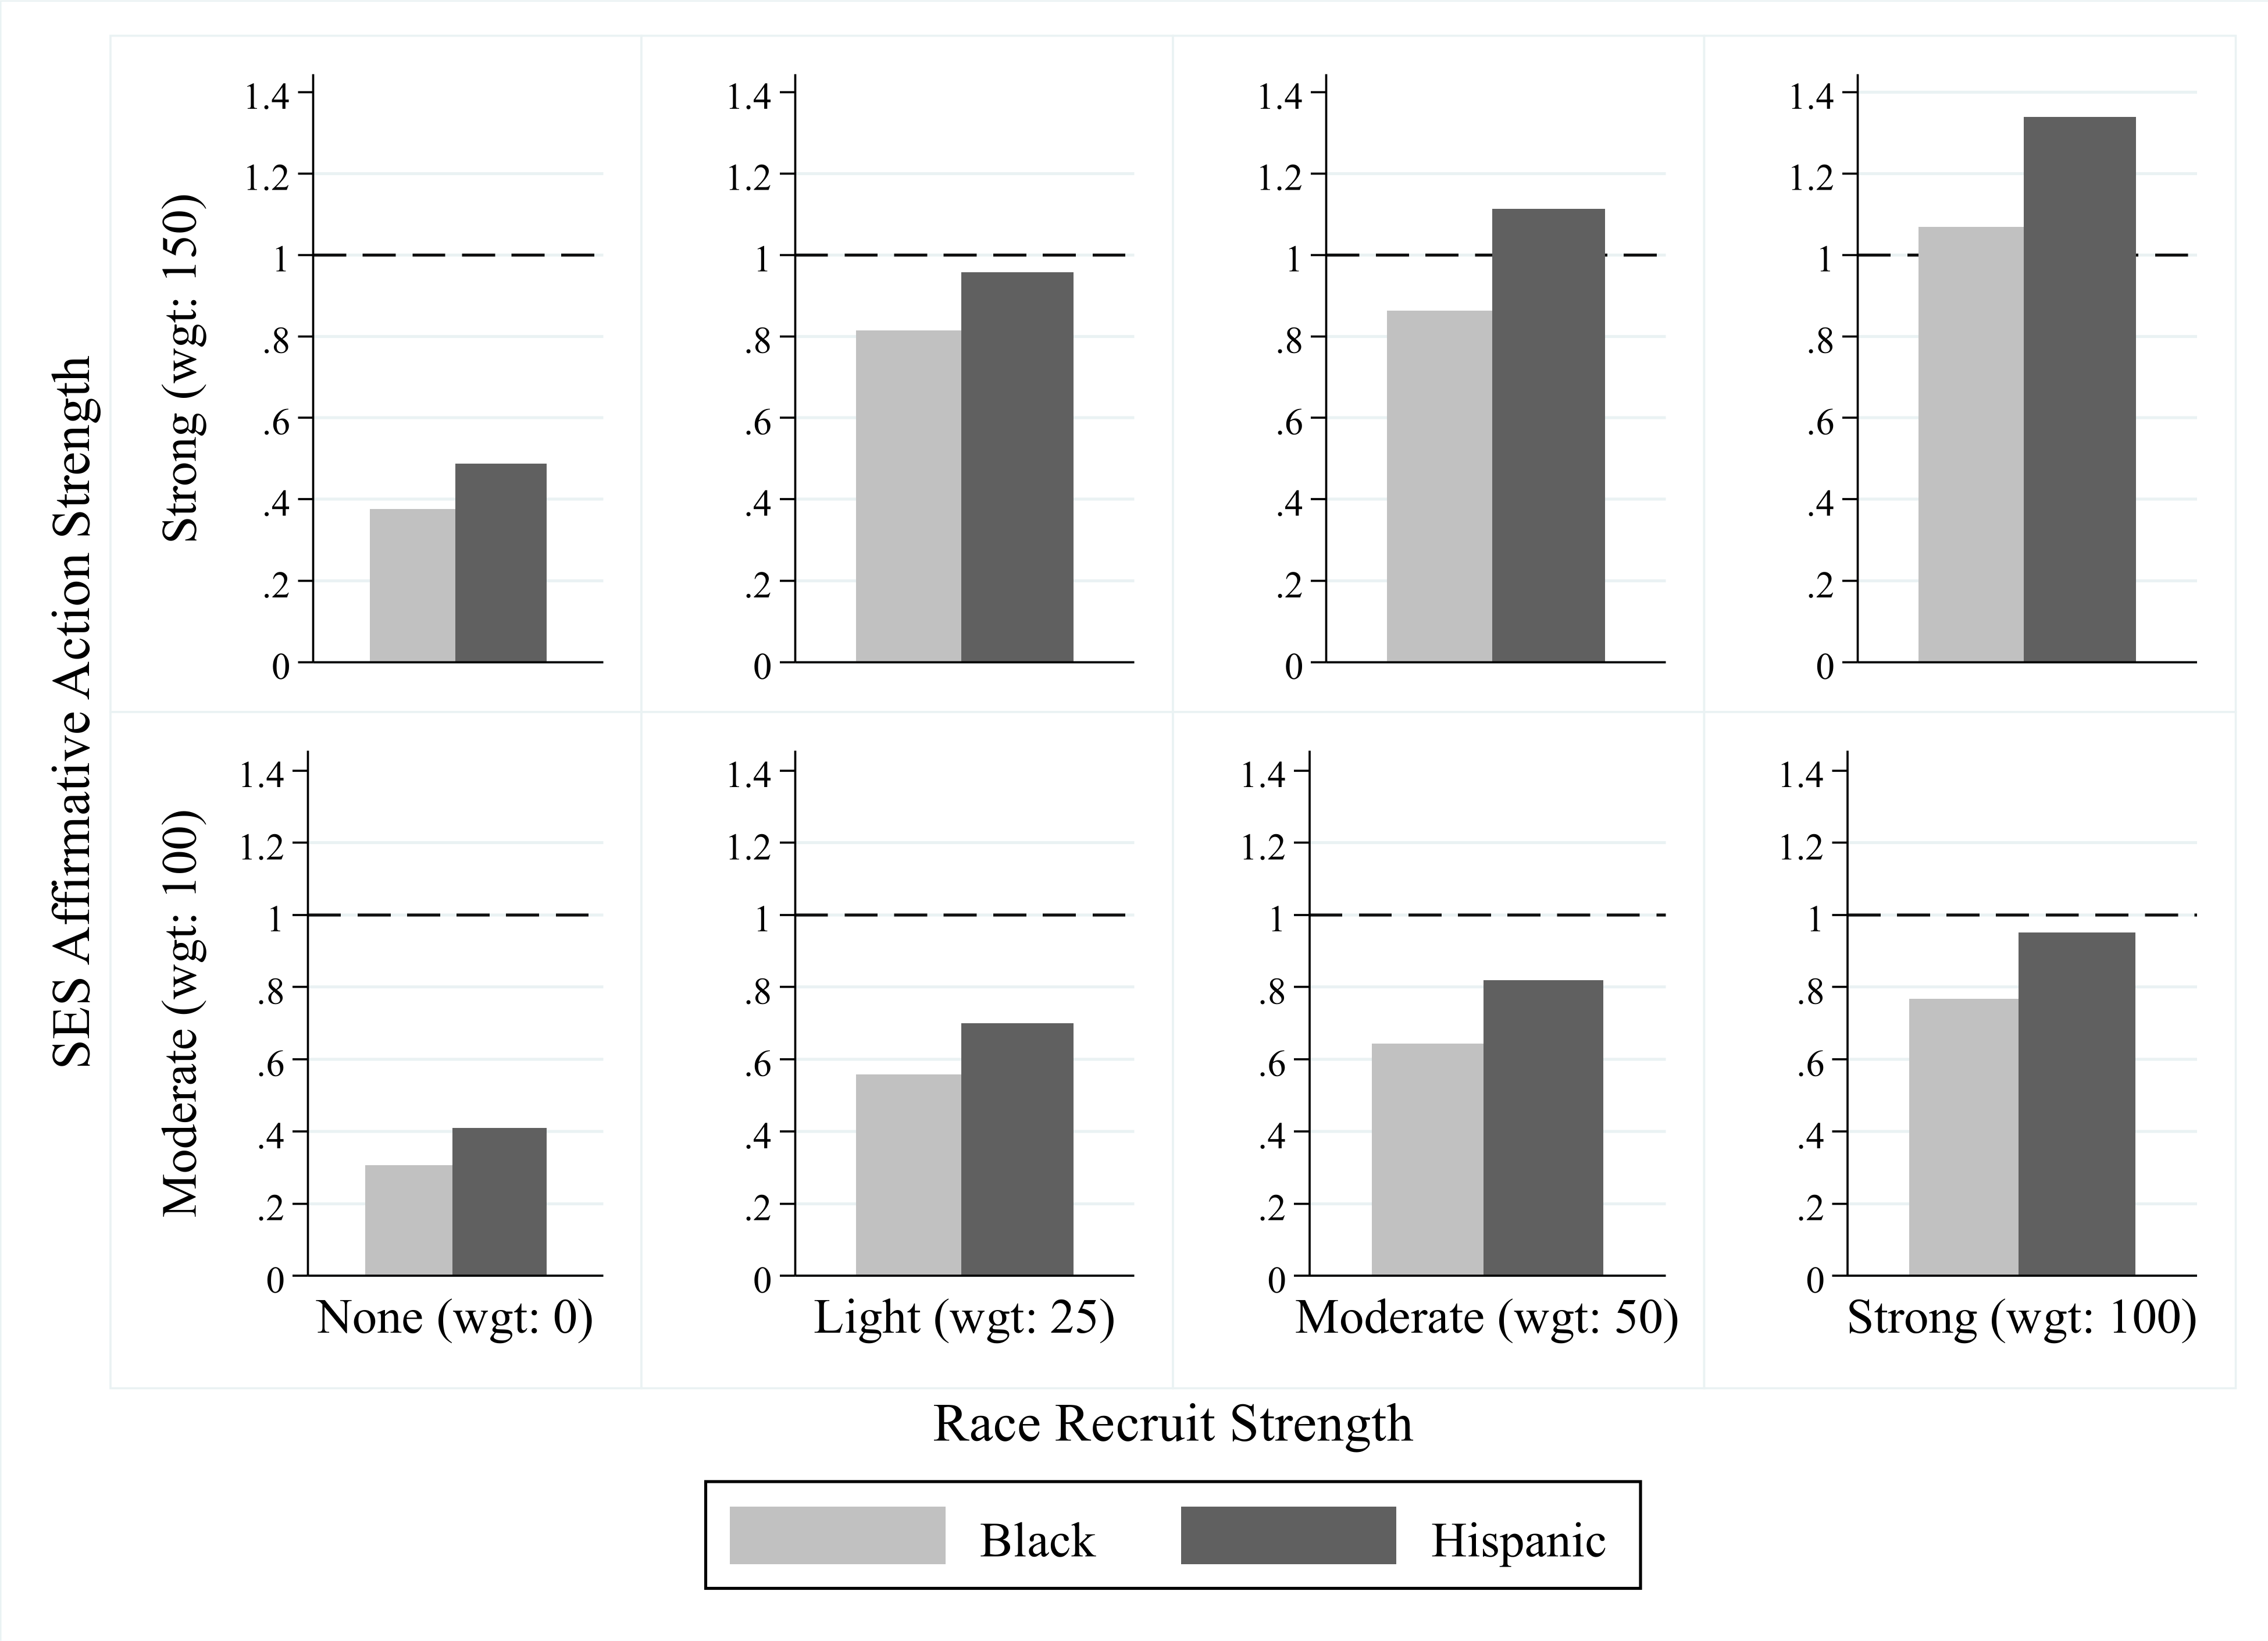
\includegraphics[width=\textwidth]{figures_original/fig2_continued.png}} \\
      %   {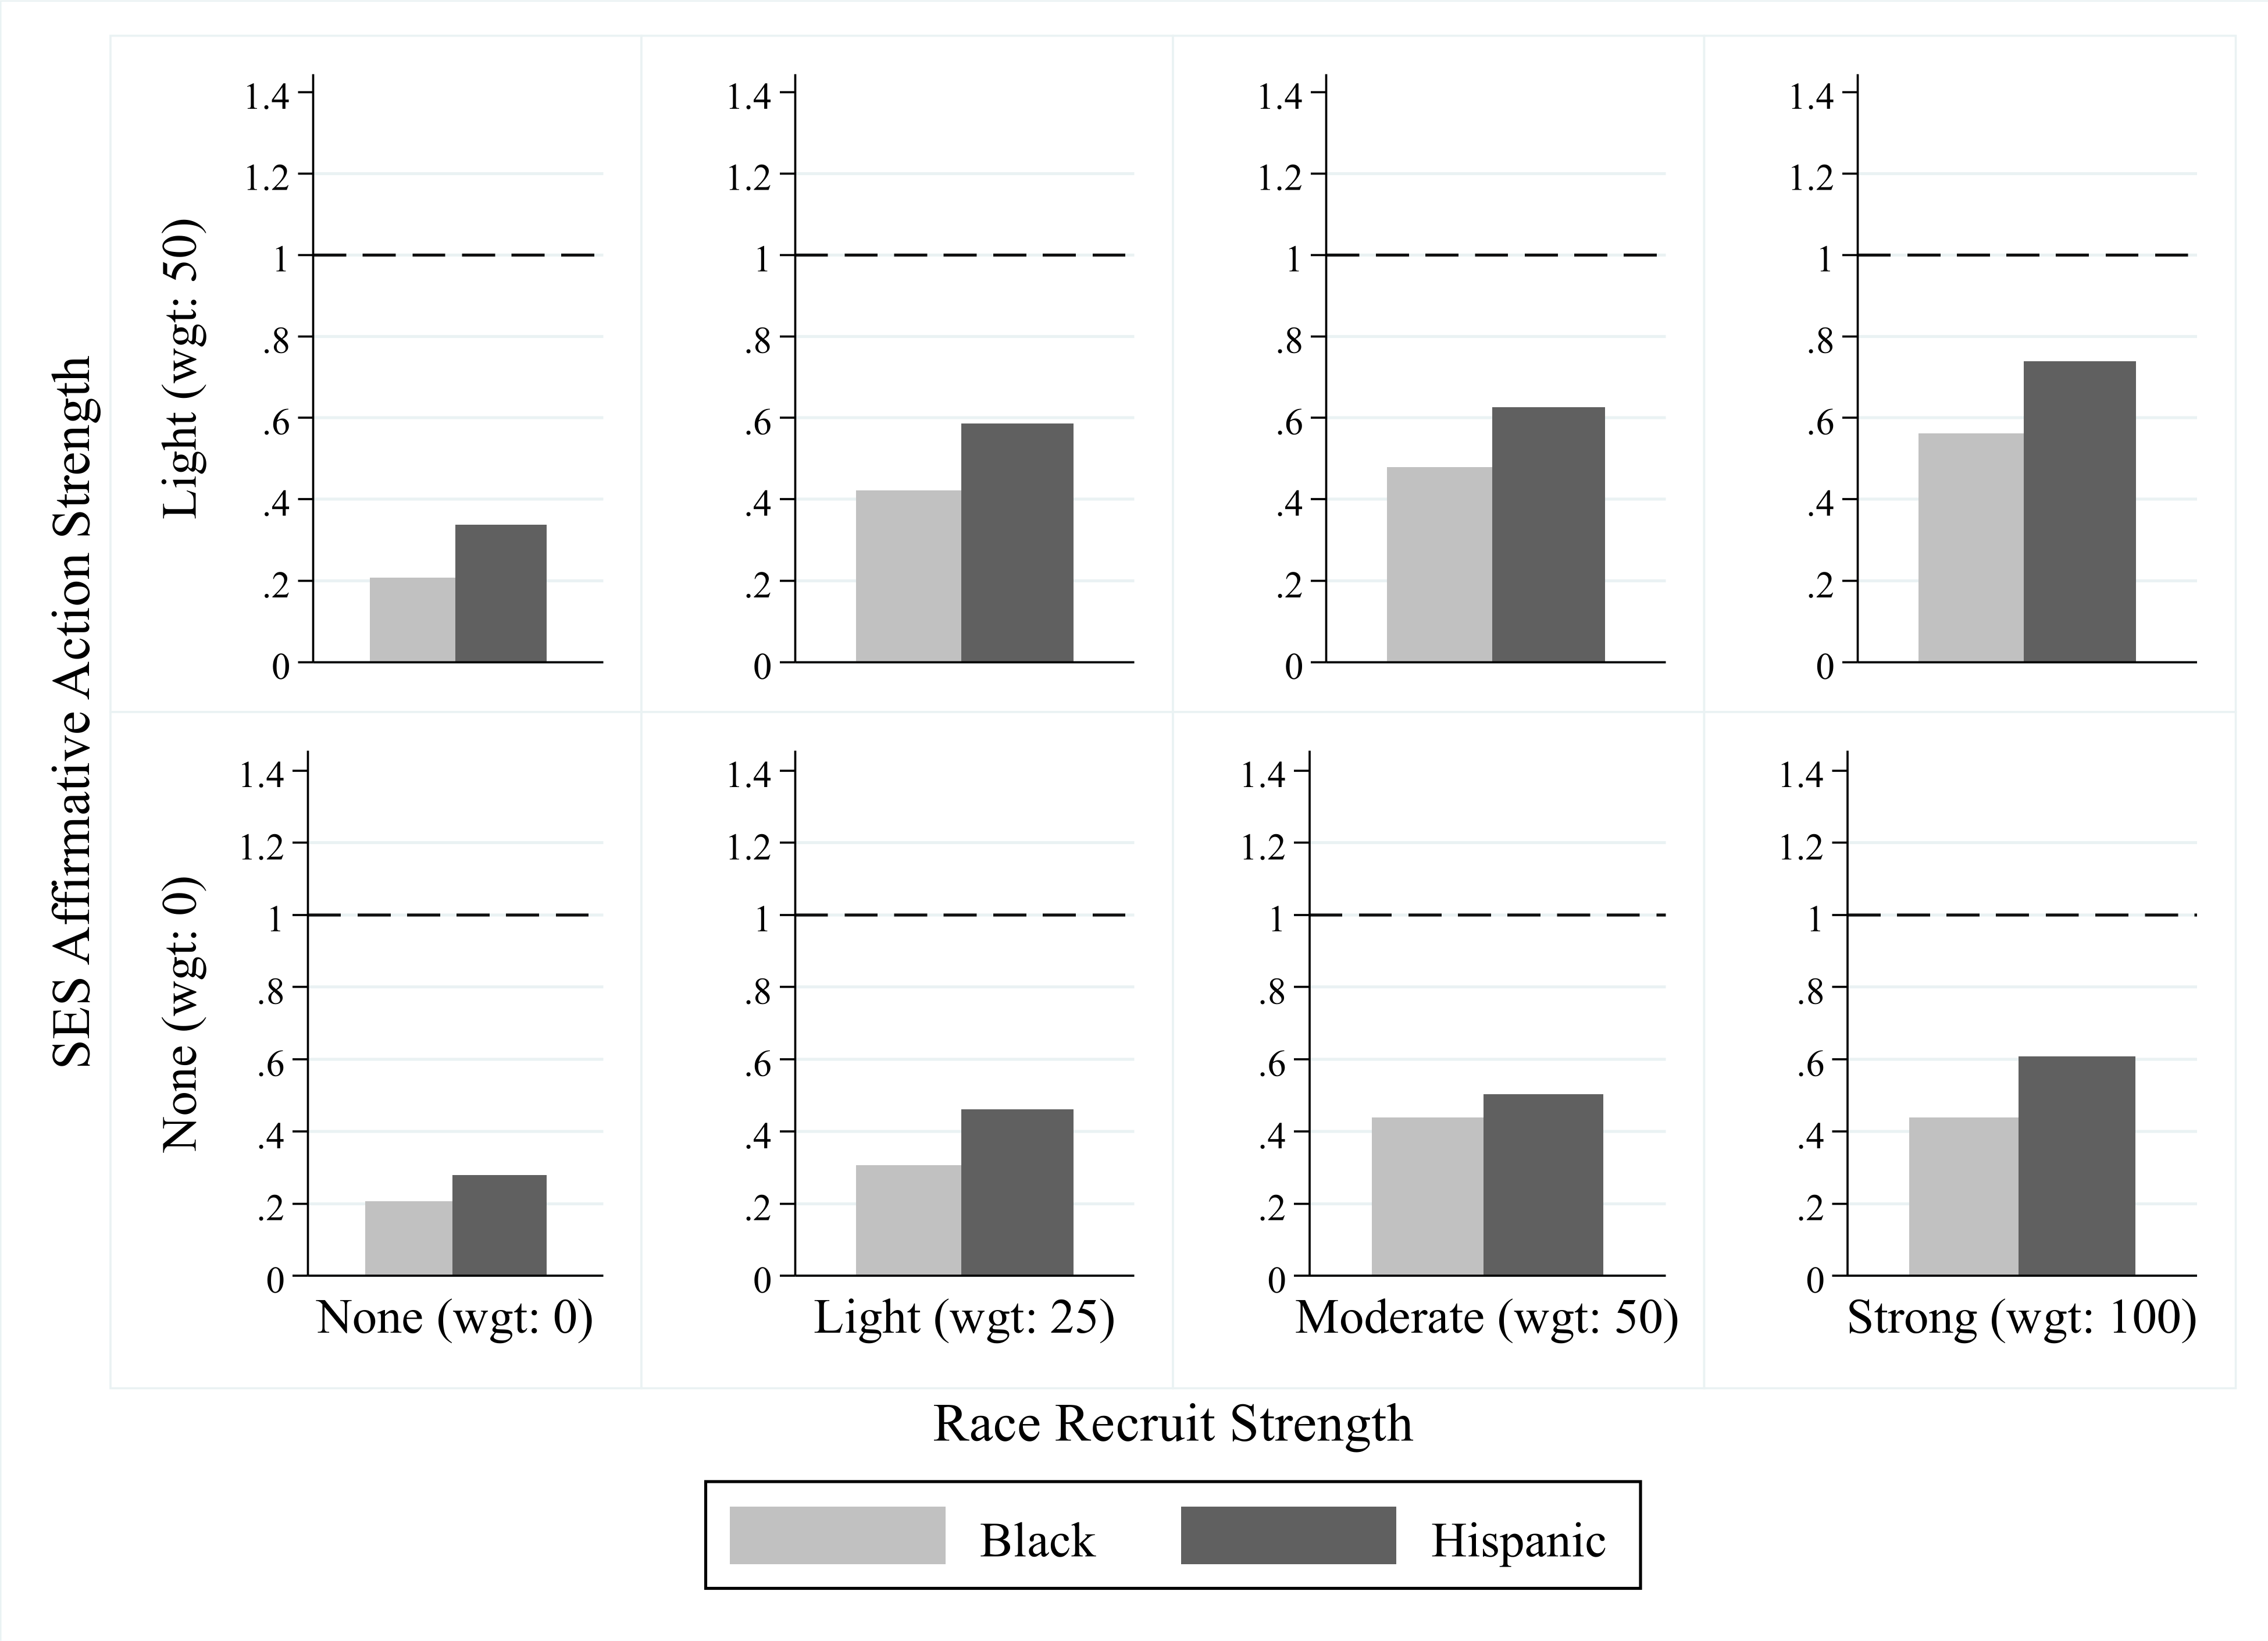
\includegraphics[width=\textwidth]{figures_original/fig2.png}}
      % }
      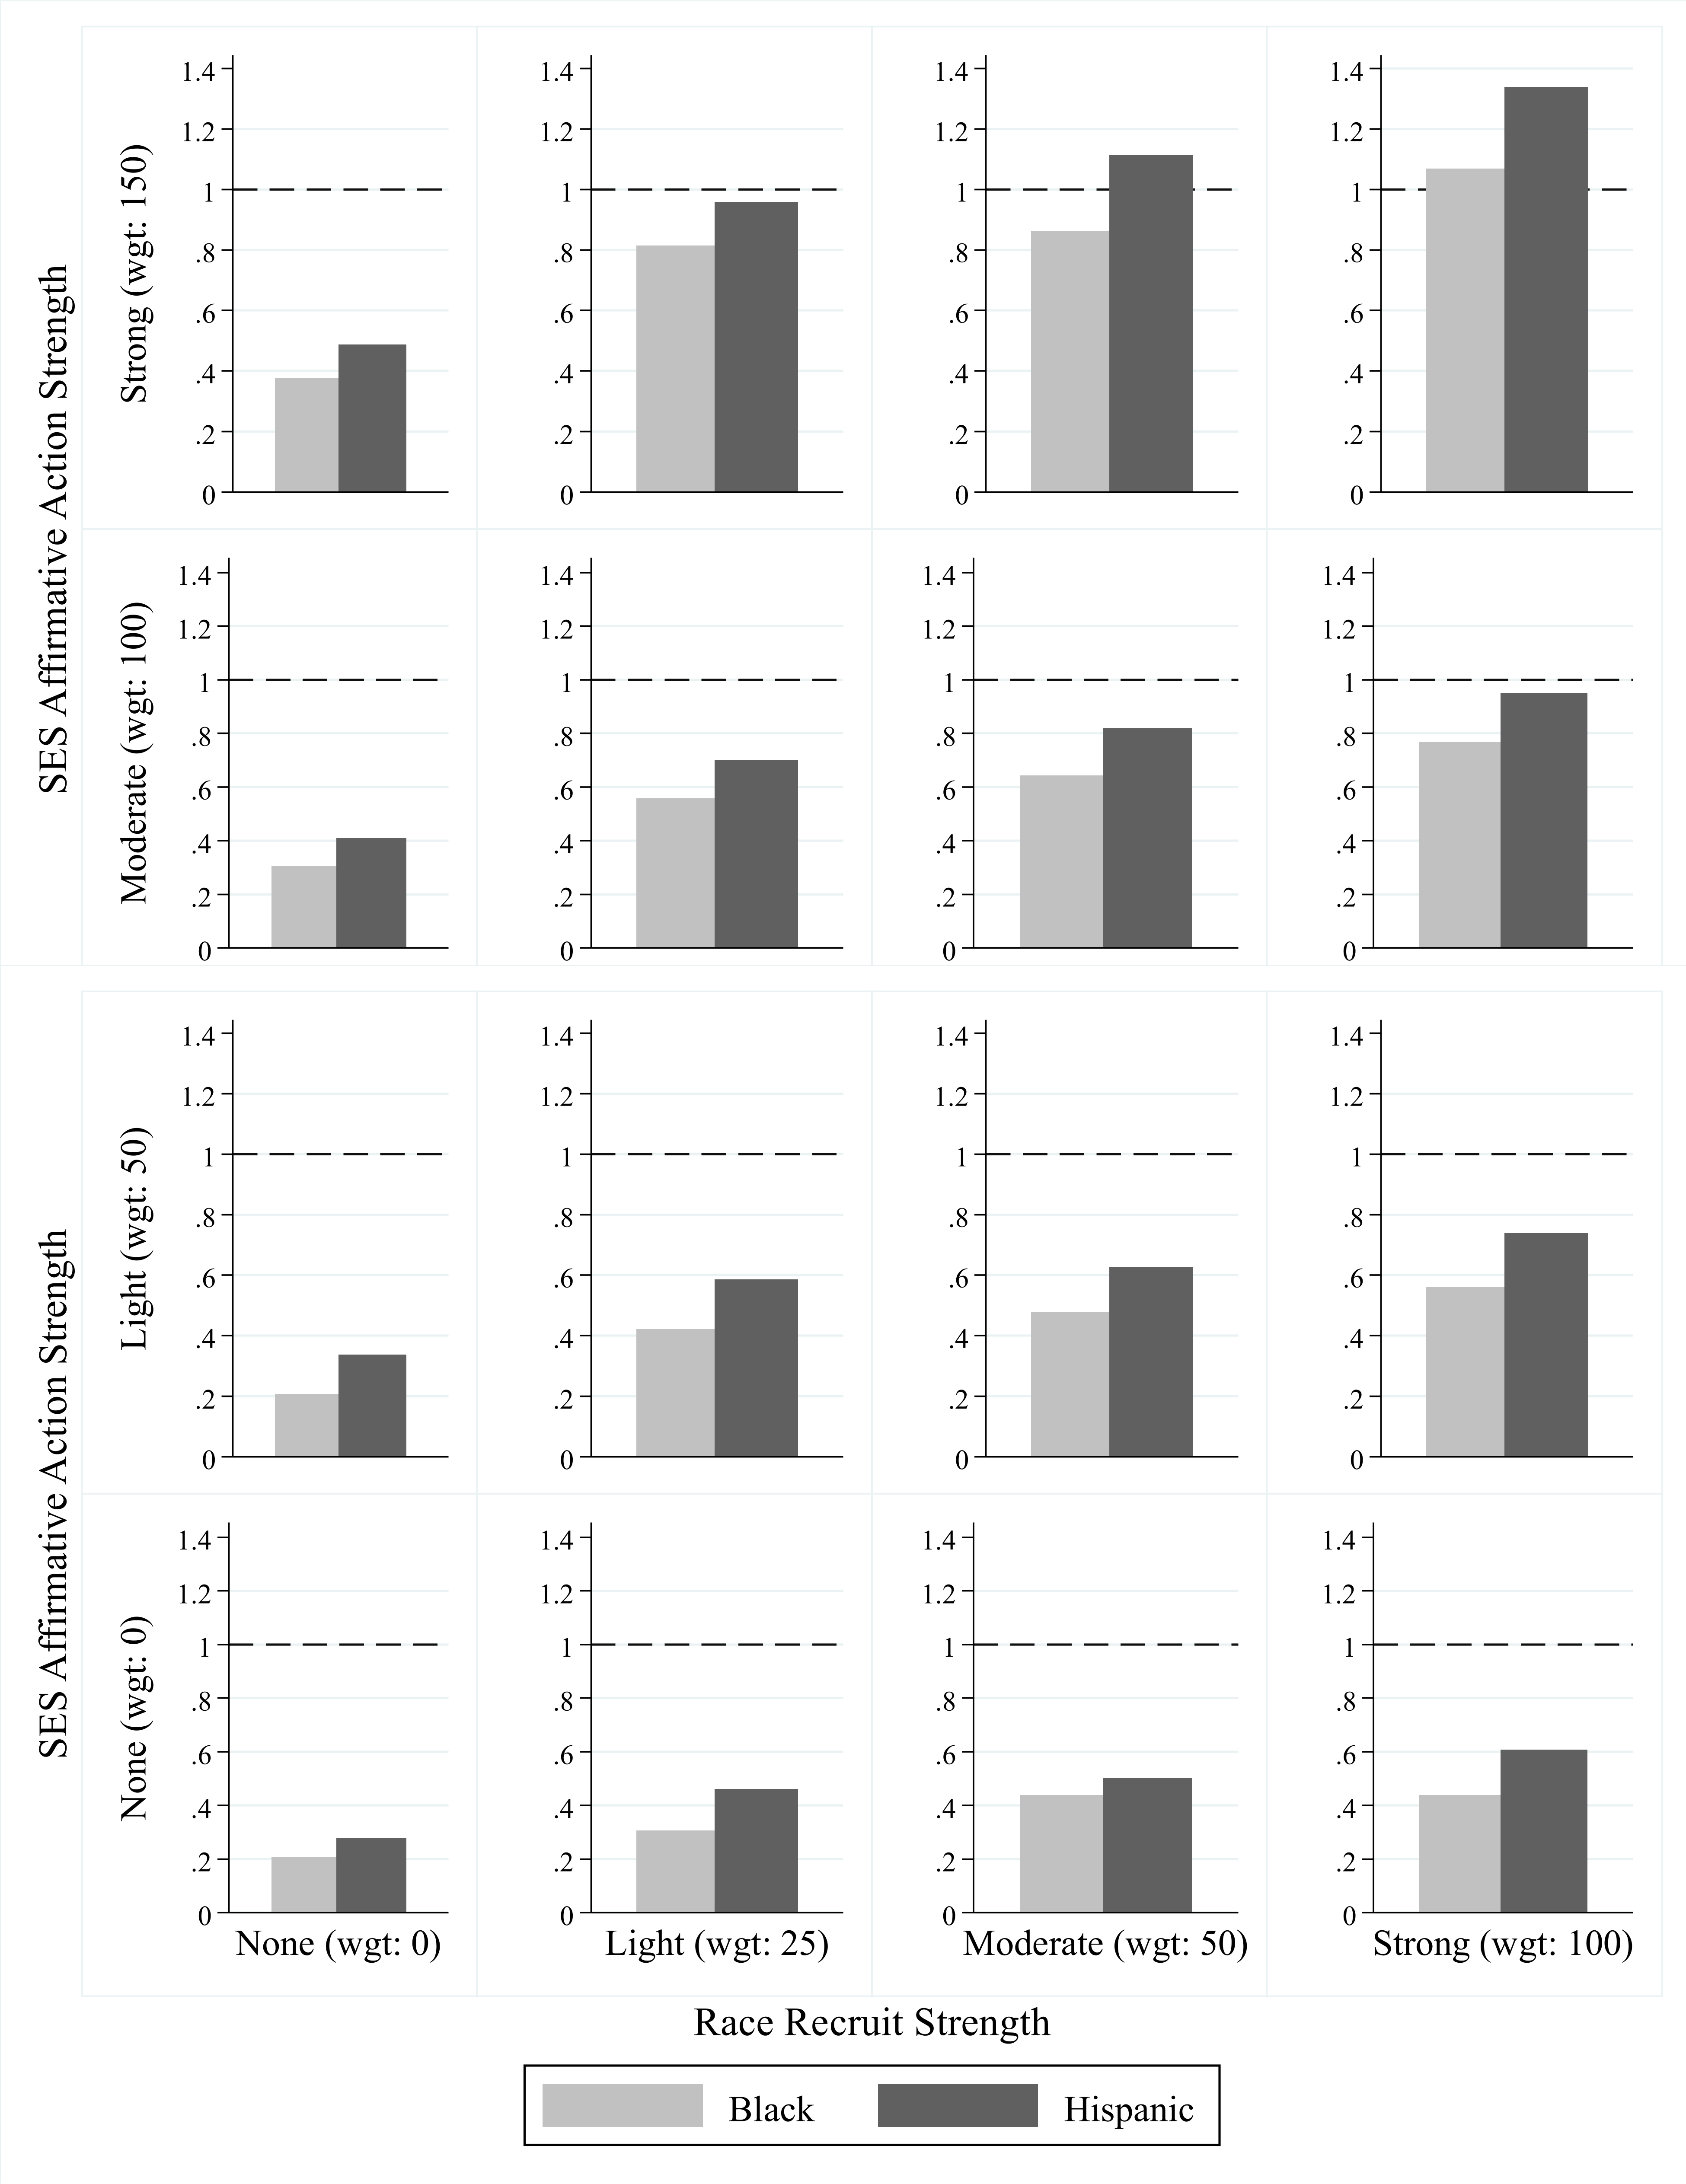
\includegraphics[width=\textwidth]{figures_original/fig2_combined.png}
    }%
  \end{minipage}%
  \hfill%
  \begin{minipage}[t]{.45\textwidth}
    \subfloat[{Replication}]{{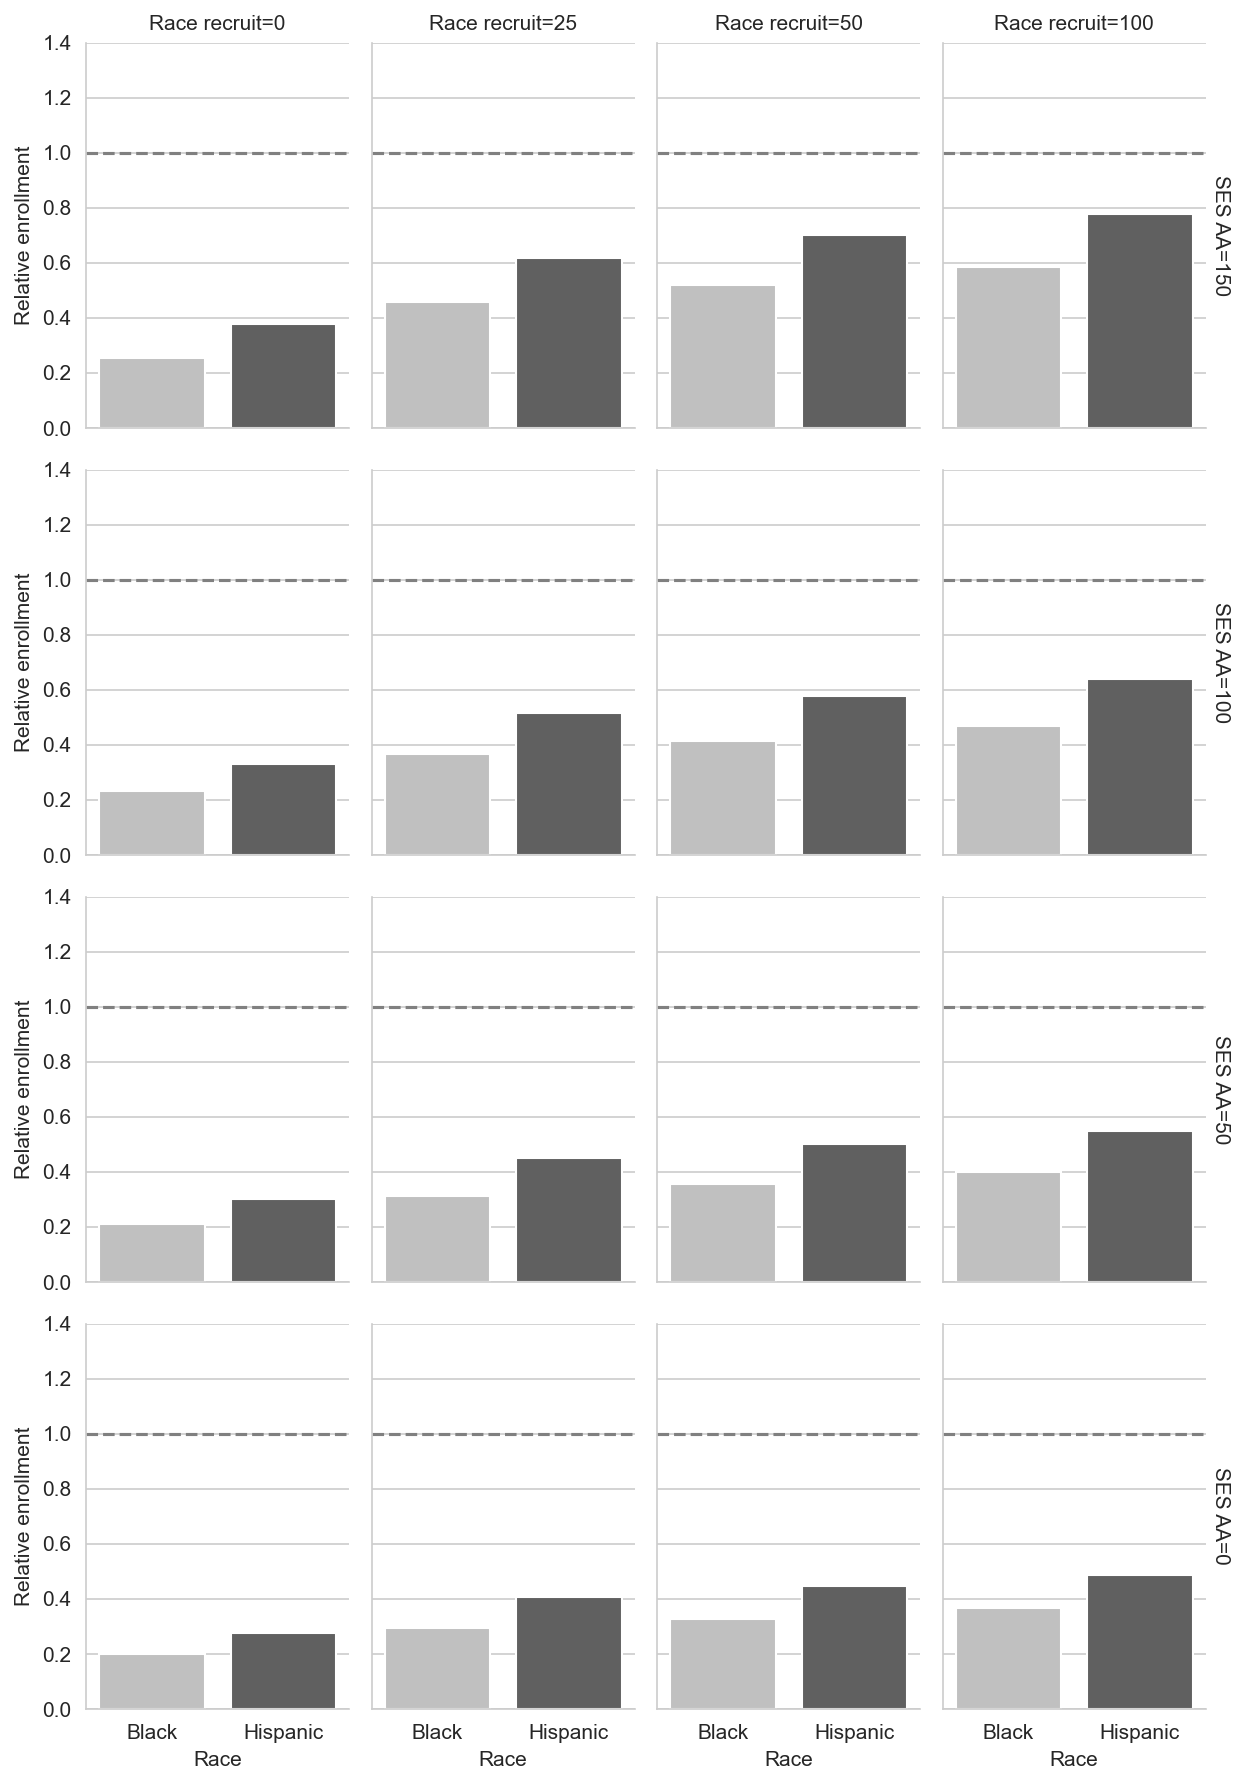
\includegraphics[width=\textwidth]{figures/fig2.png}}}
  \end{minipage}%
  \caption{Black and Hispanic enrollment in colleges using SES-based affirmative action and race-based recruitment, as a share of estimated enrollment under race-based affirmative action (using estimated real-world affirmative action weight 260).}
  \label{fig:2}
\end{figure}

\begin{figure}[p]
  \centering
  \subfloat[{Original (reprinted from~\cite[Figure~A2]{reardon2018levels_preprint})}]{{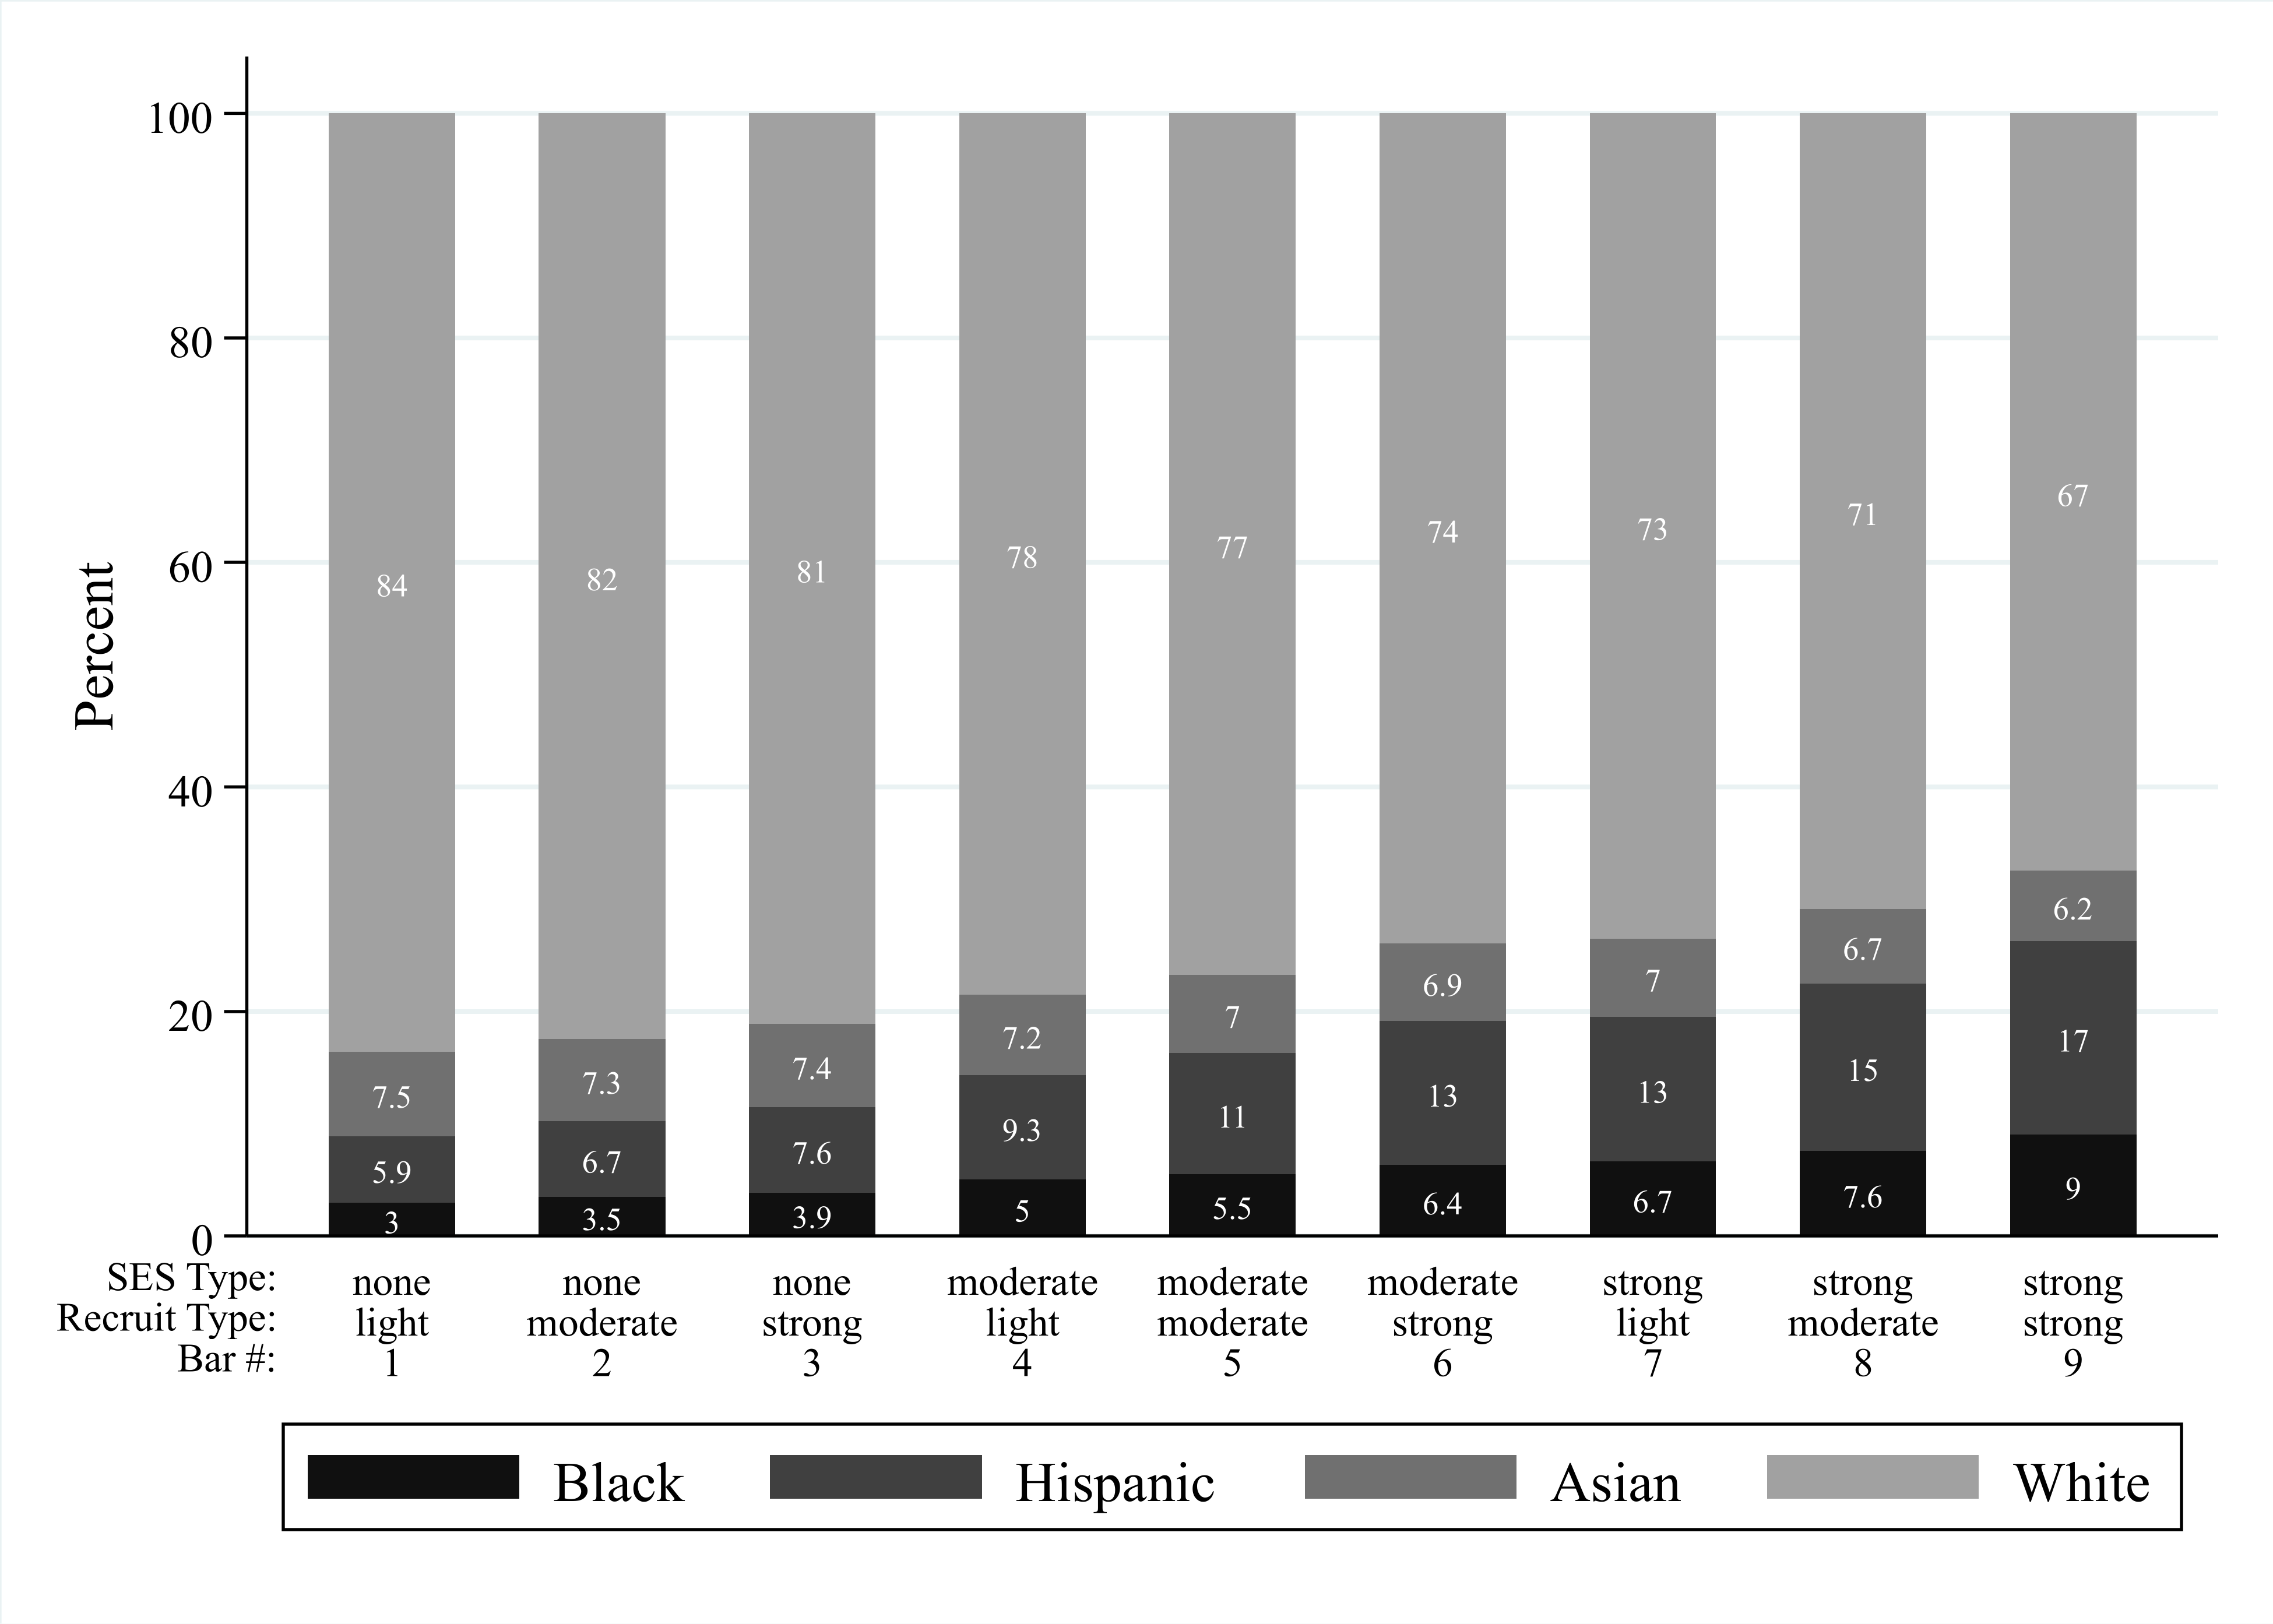
\includegraphics[width=.49\textwidth]{figures_original/figA2.png}}}
  \hfill
  \subfloat[{Reproduction}]{{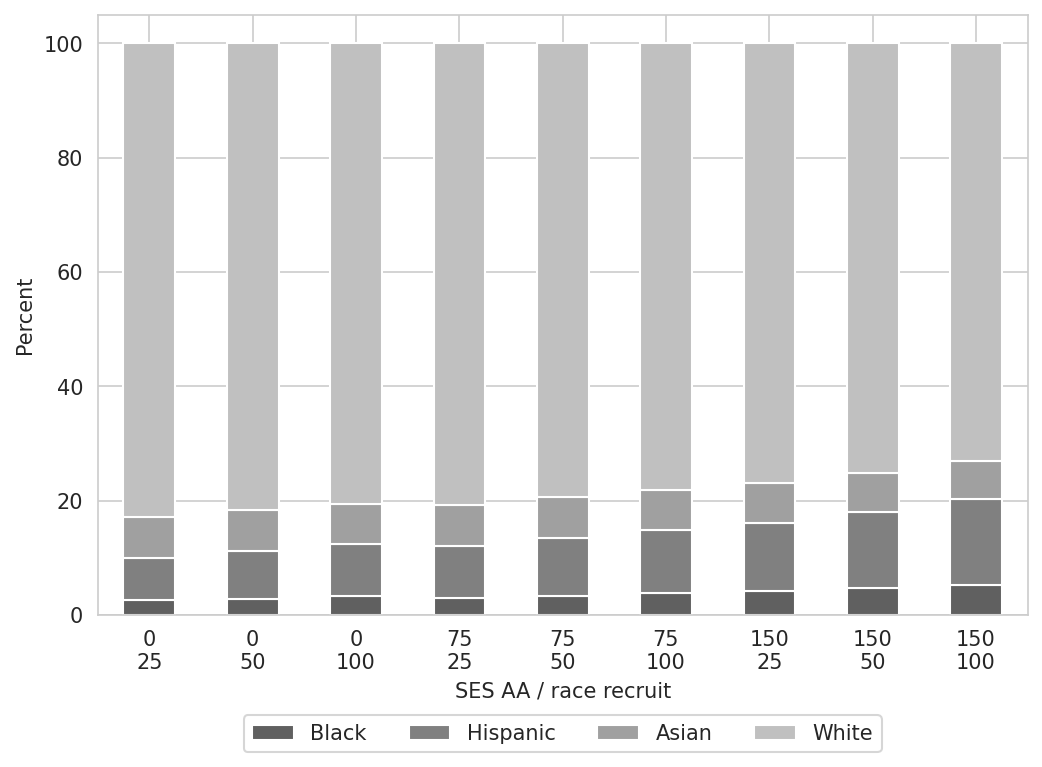
\includegraphics[width=.49\textwidth]{figures/figA2.png}}}
  \caption{Racial composition of colleges using SES-based affirmative
    action and race-based recruitment, by affirmative action and
    recruitment weights.}
  \label{fig:A2}
\end{figure}

\begin{figure}[p]
  \centering
  \subfloat[{Original (reprinted from~\cite[Figure~A3]{reardon2018levels_preprint})}]{{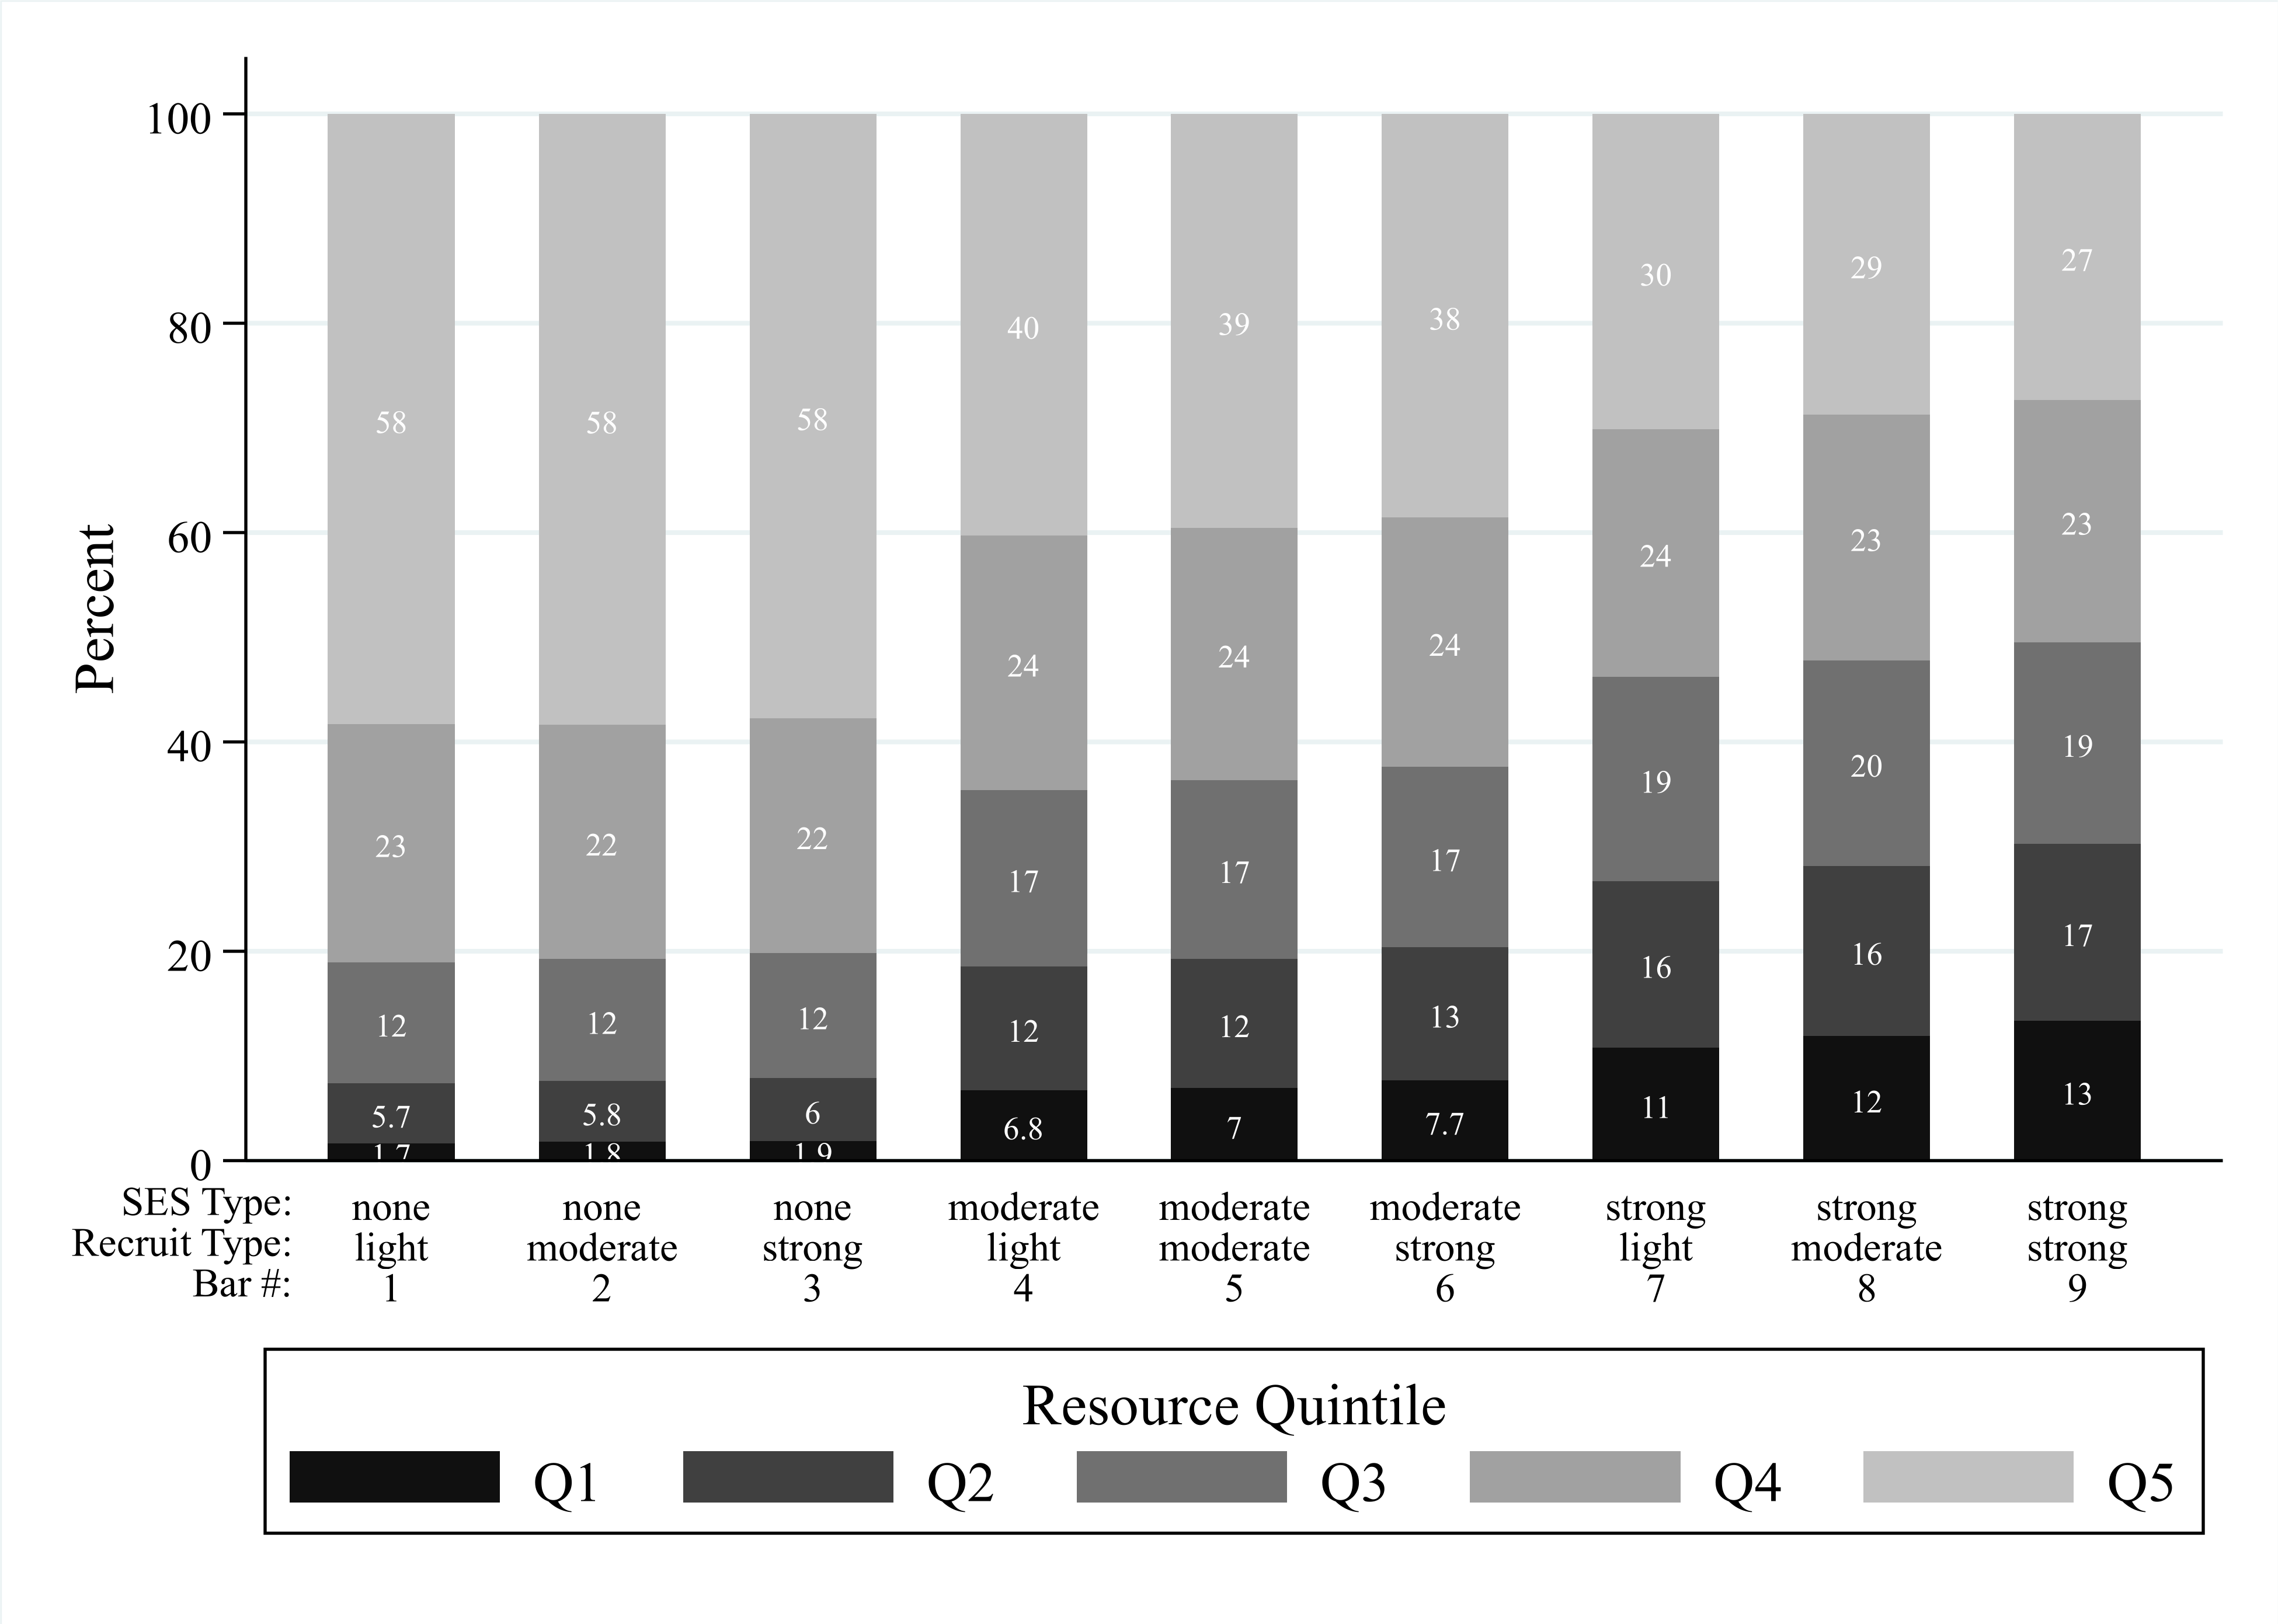
\includegraphics[width=.49\textwidth]{figures_original/figA3.png}}}
  \hfill
  \subfloat[{Reproduction}]{{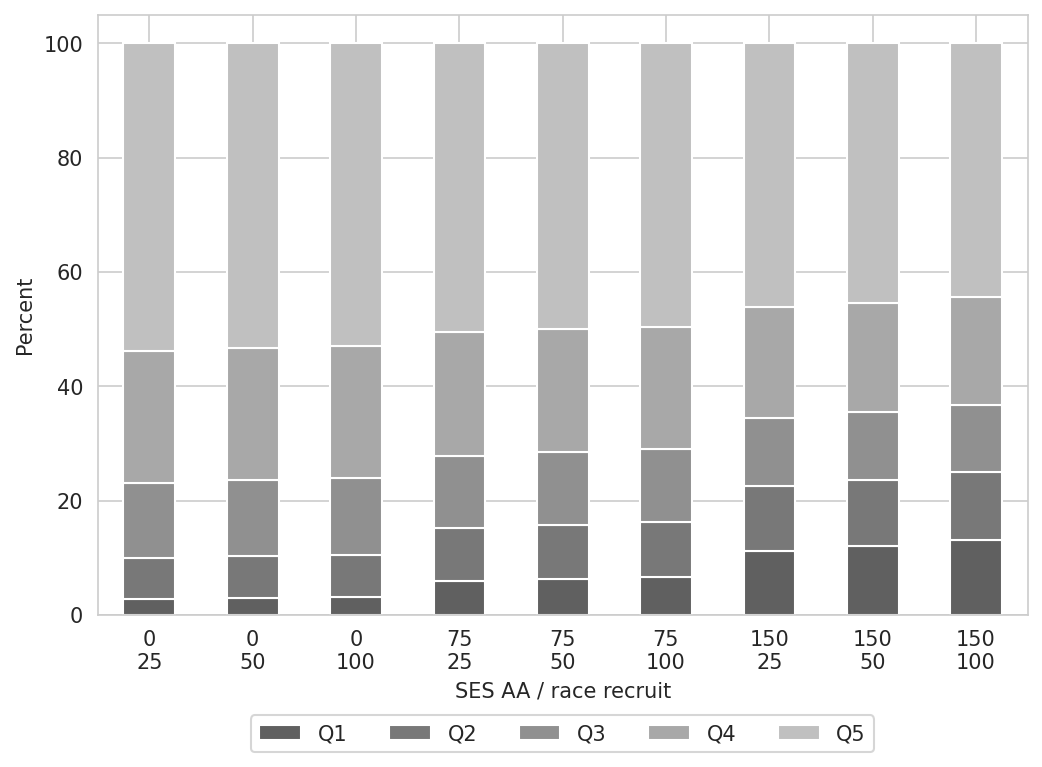
\includegraphics[width=.49\textwidth]{figures/figA3.png}}}
  \caption{Socioeconomic composition of colleges using SES-based
    affirmative action and race-based recruitment, by affirmative
    action and recruitment weights.}
  \label{fig:A3}
\end{figure}

\begin{figure}[p]
  \centering
  \subfloat[{Original (reprinted from~\cite[Figure~A4]{reardon2018levels_preprint})}]{{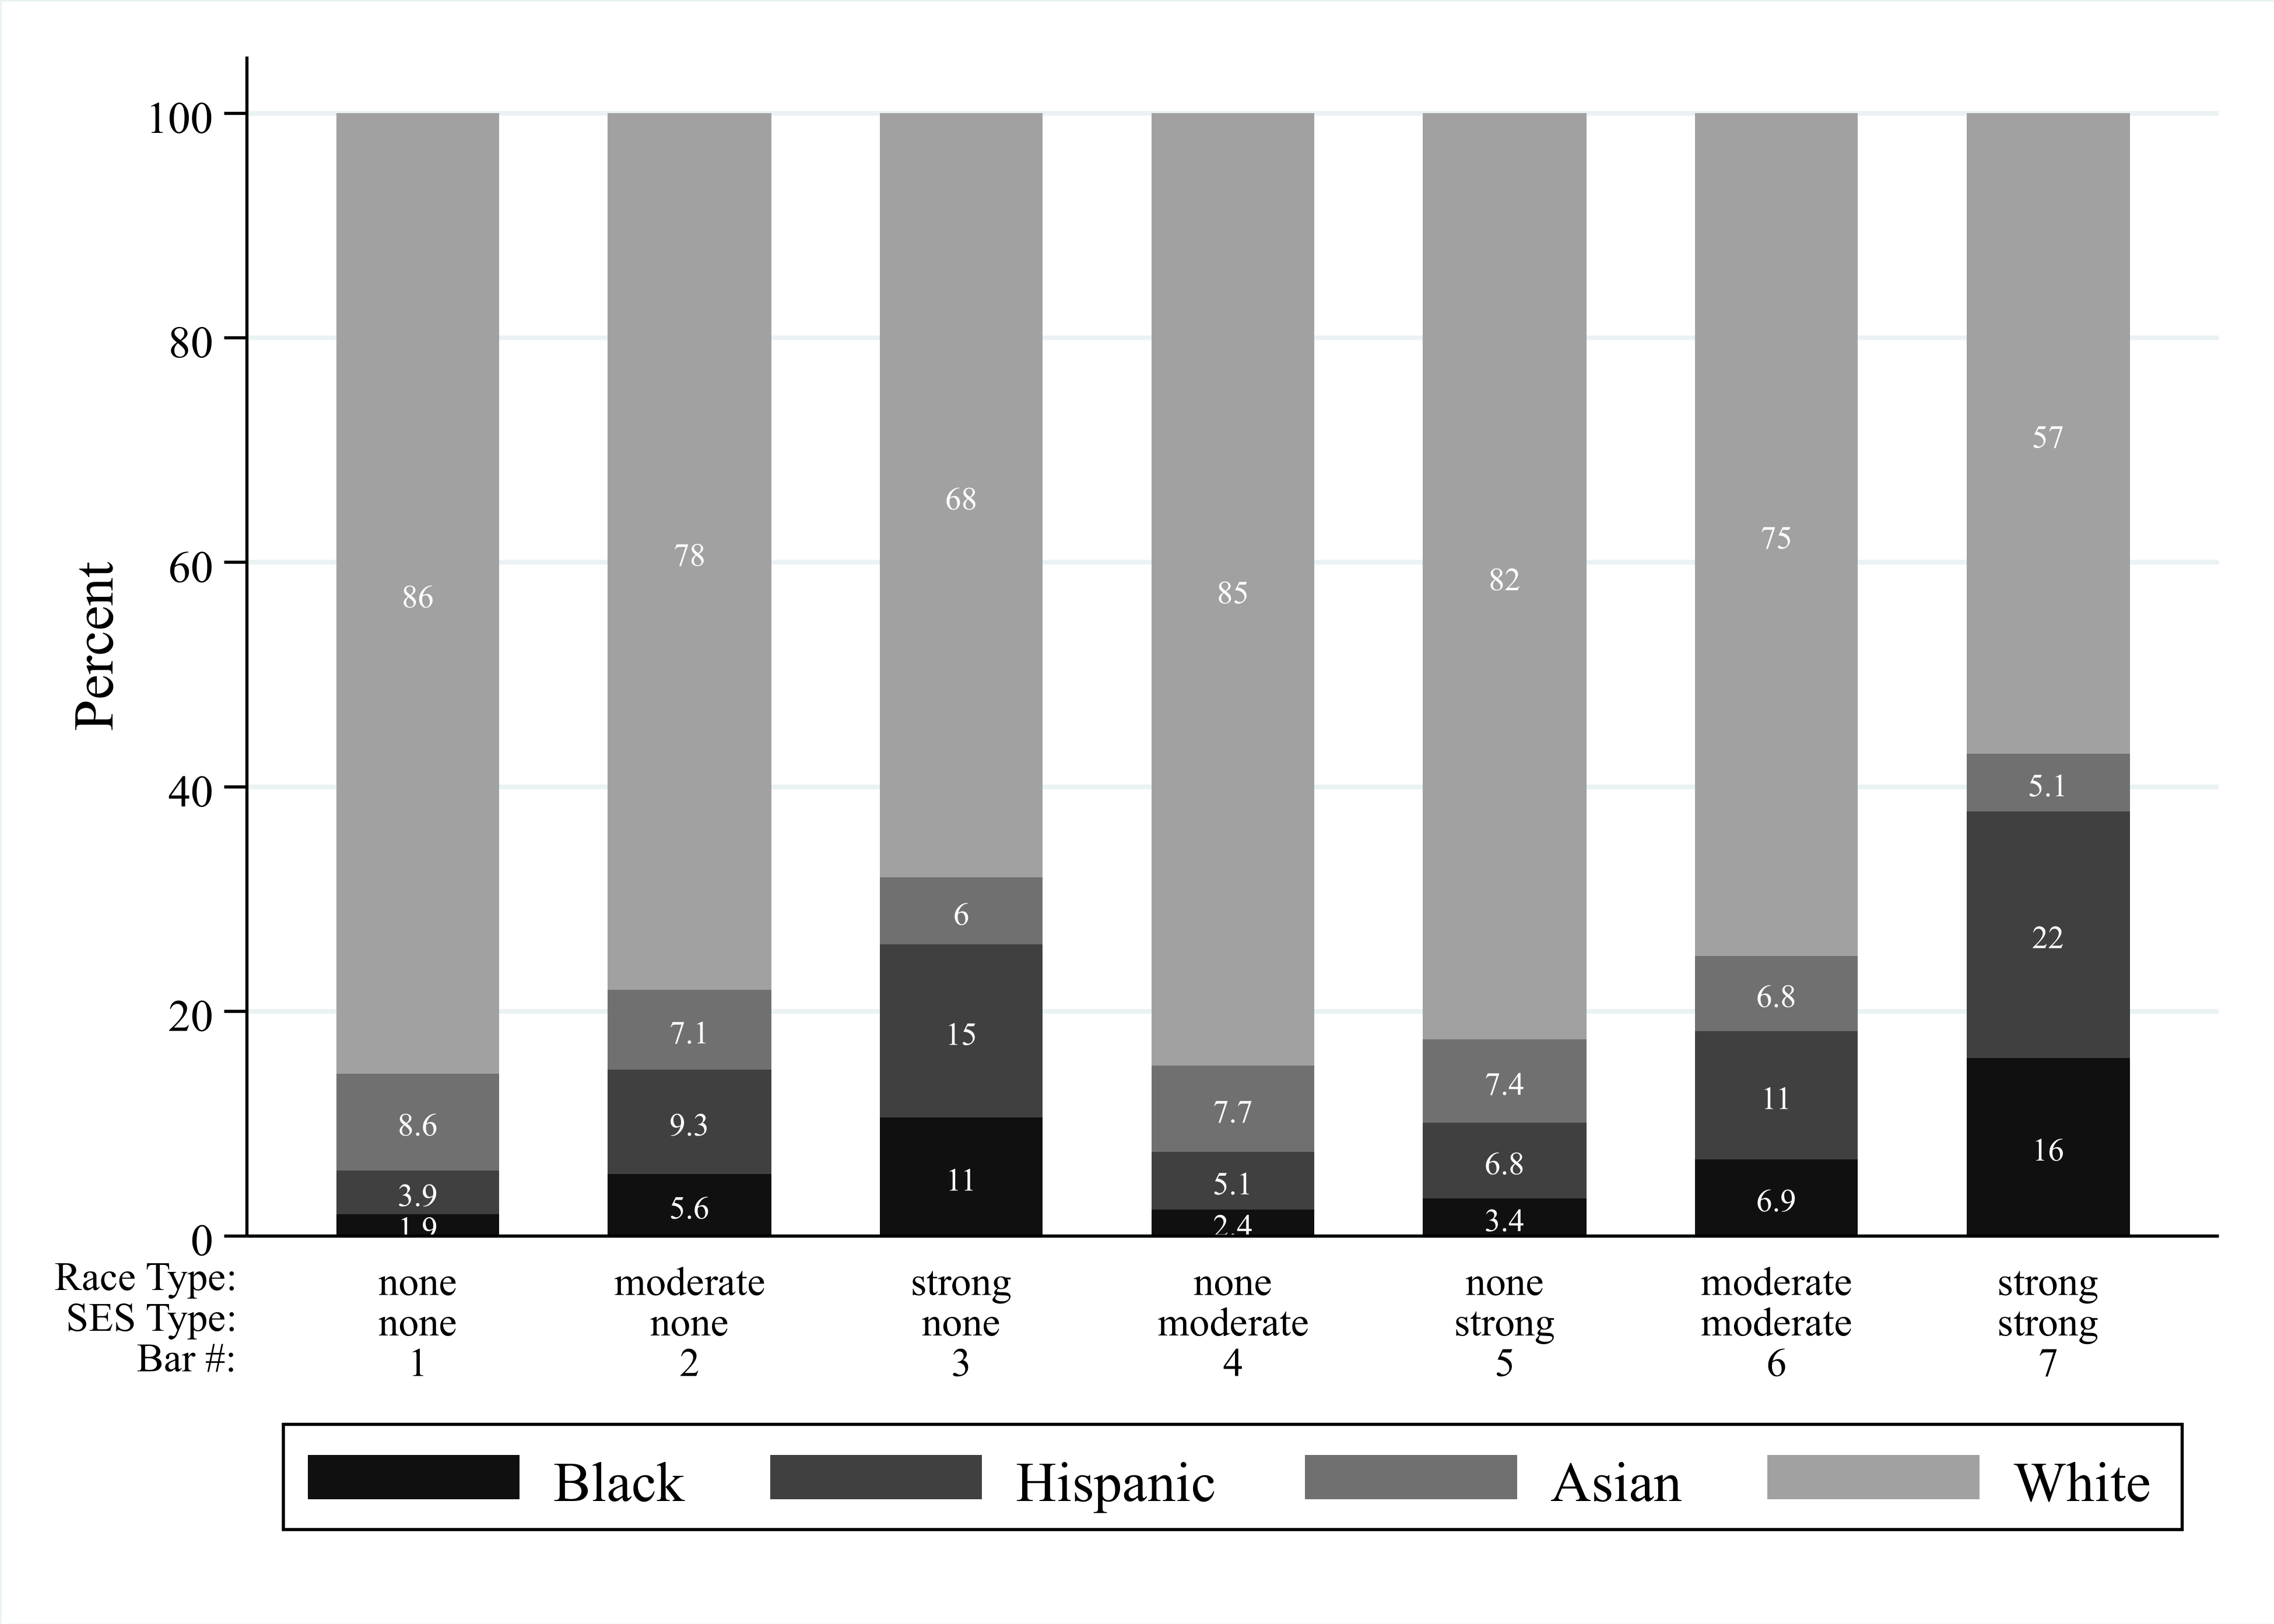
\includegraphics[width=.49\textwidth]{figures_original/figA4.png}}}
  \hfill
  \subfloat[{Reproduction: racial composition}]{{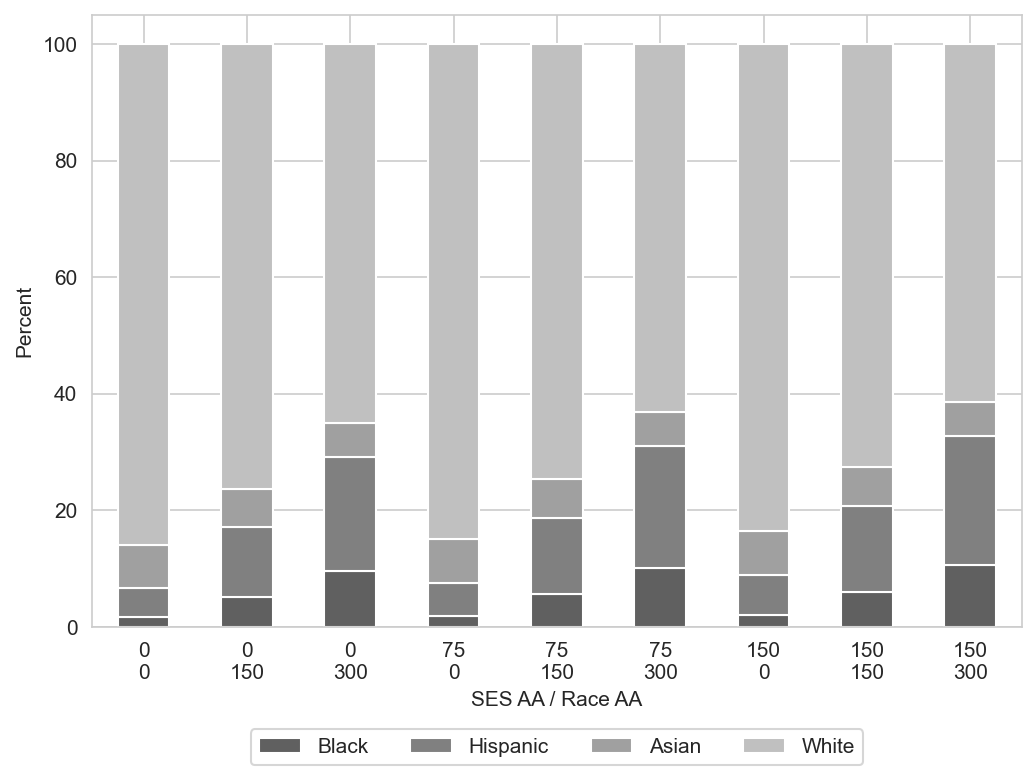
\includegraphics[width=.49\textwidth]{figures/figA4.png}}}
  \caption{Racial composition of colleges using SES-based and racial
    affirmative actions, by affirmative action weights.}
  \label{fig:A4}
\end{figure}

\begin{figure}[p]
  \centering
  \subfloat[{Original (reprinted from~\cite[Figure~A5]{reardon2018levels_preprint})}]{{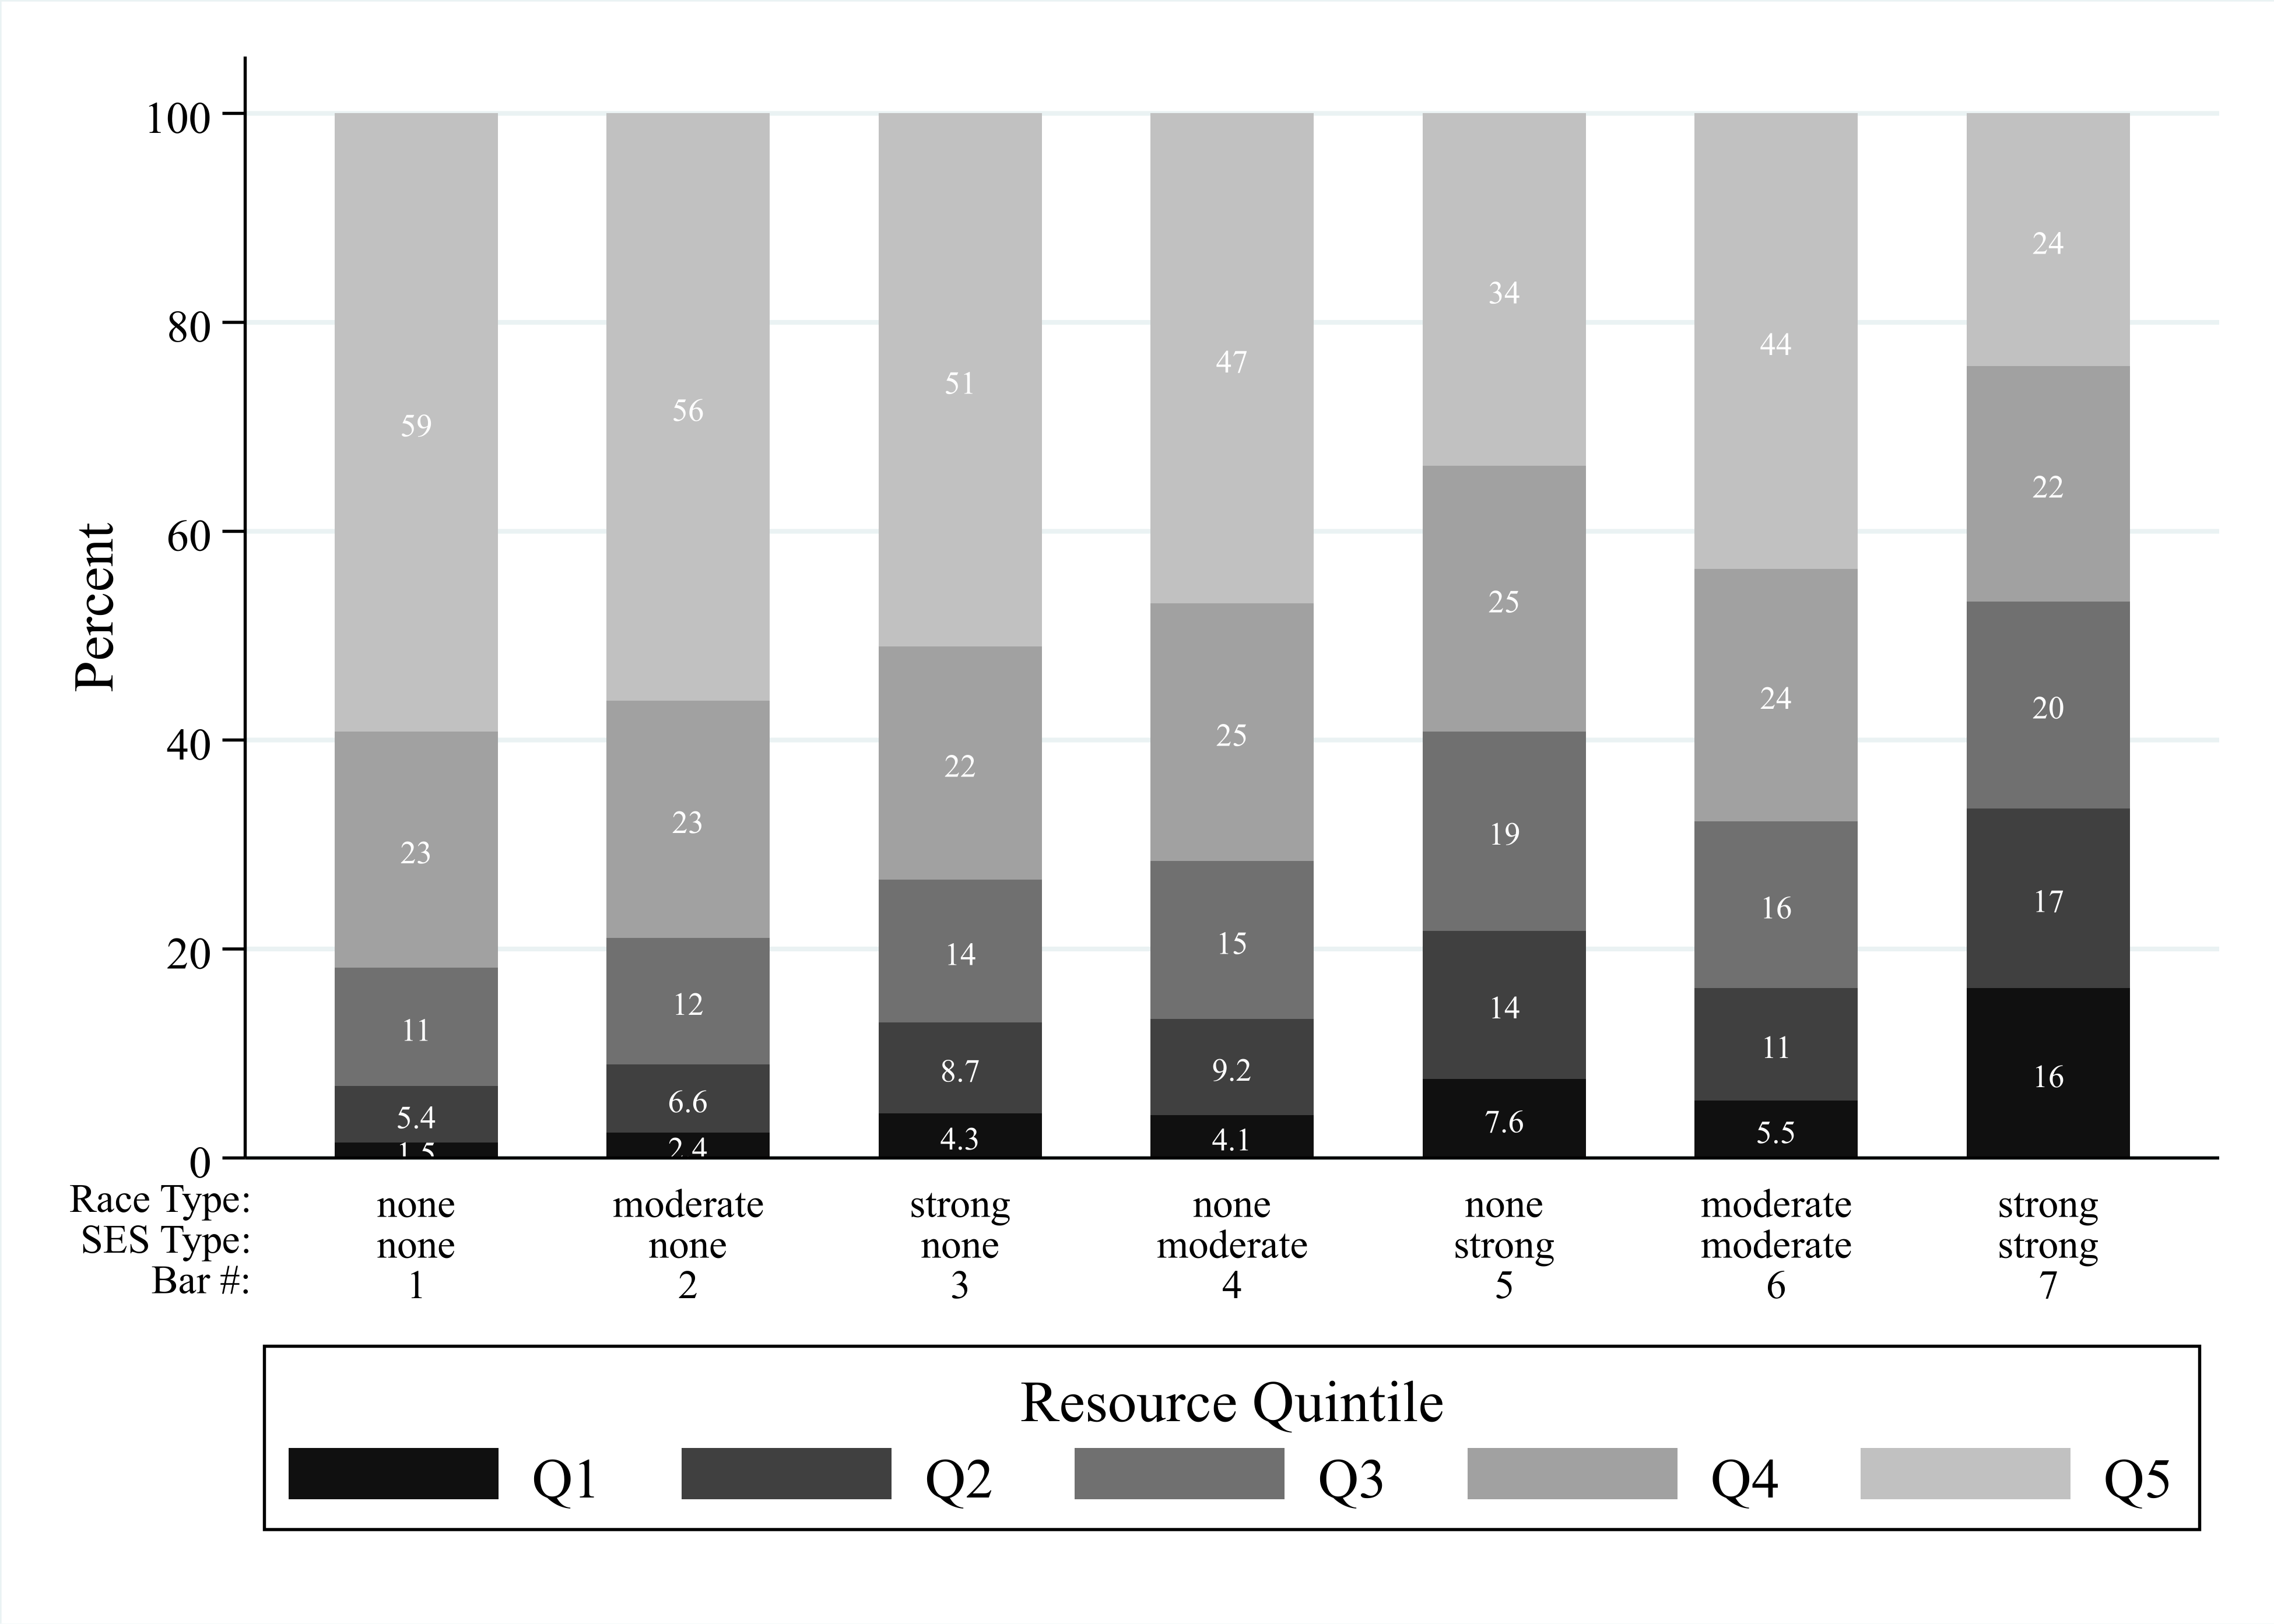
\includegraphics[width=.49\textwidth]{figures_original/figA5.png}}}
  \hfill
  \subfloat[{Reproduction}]{{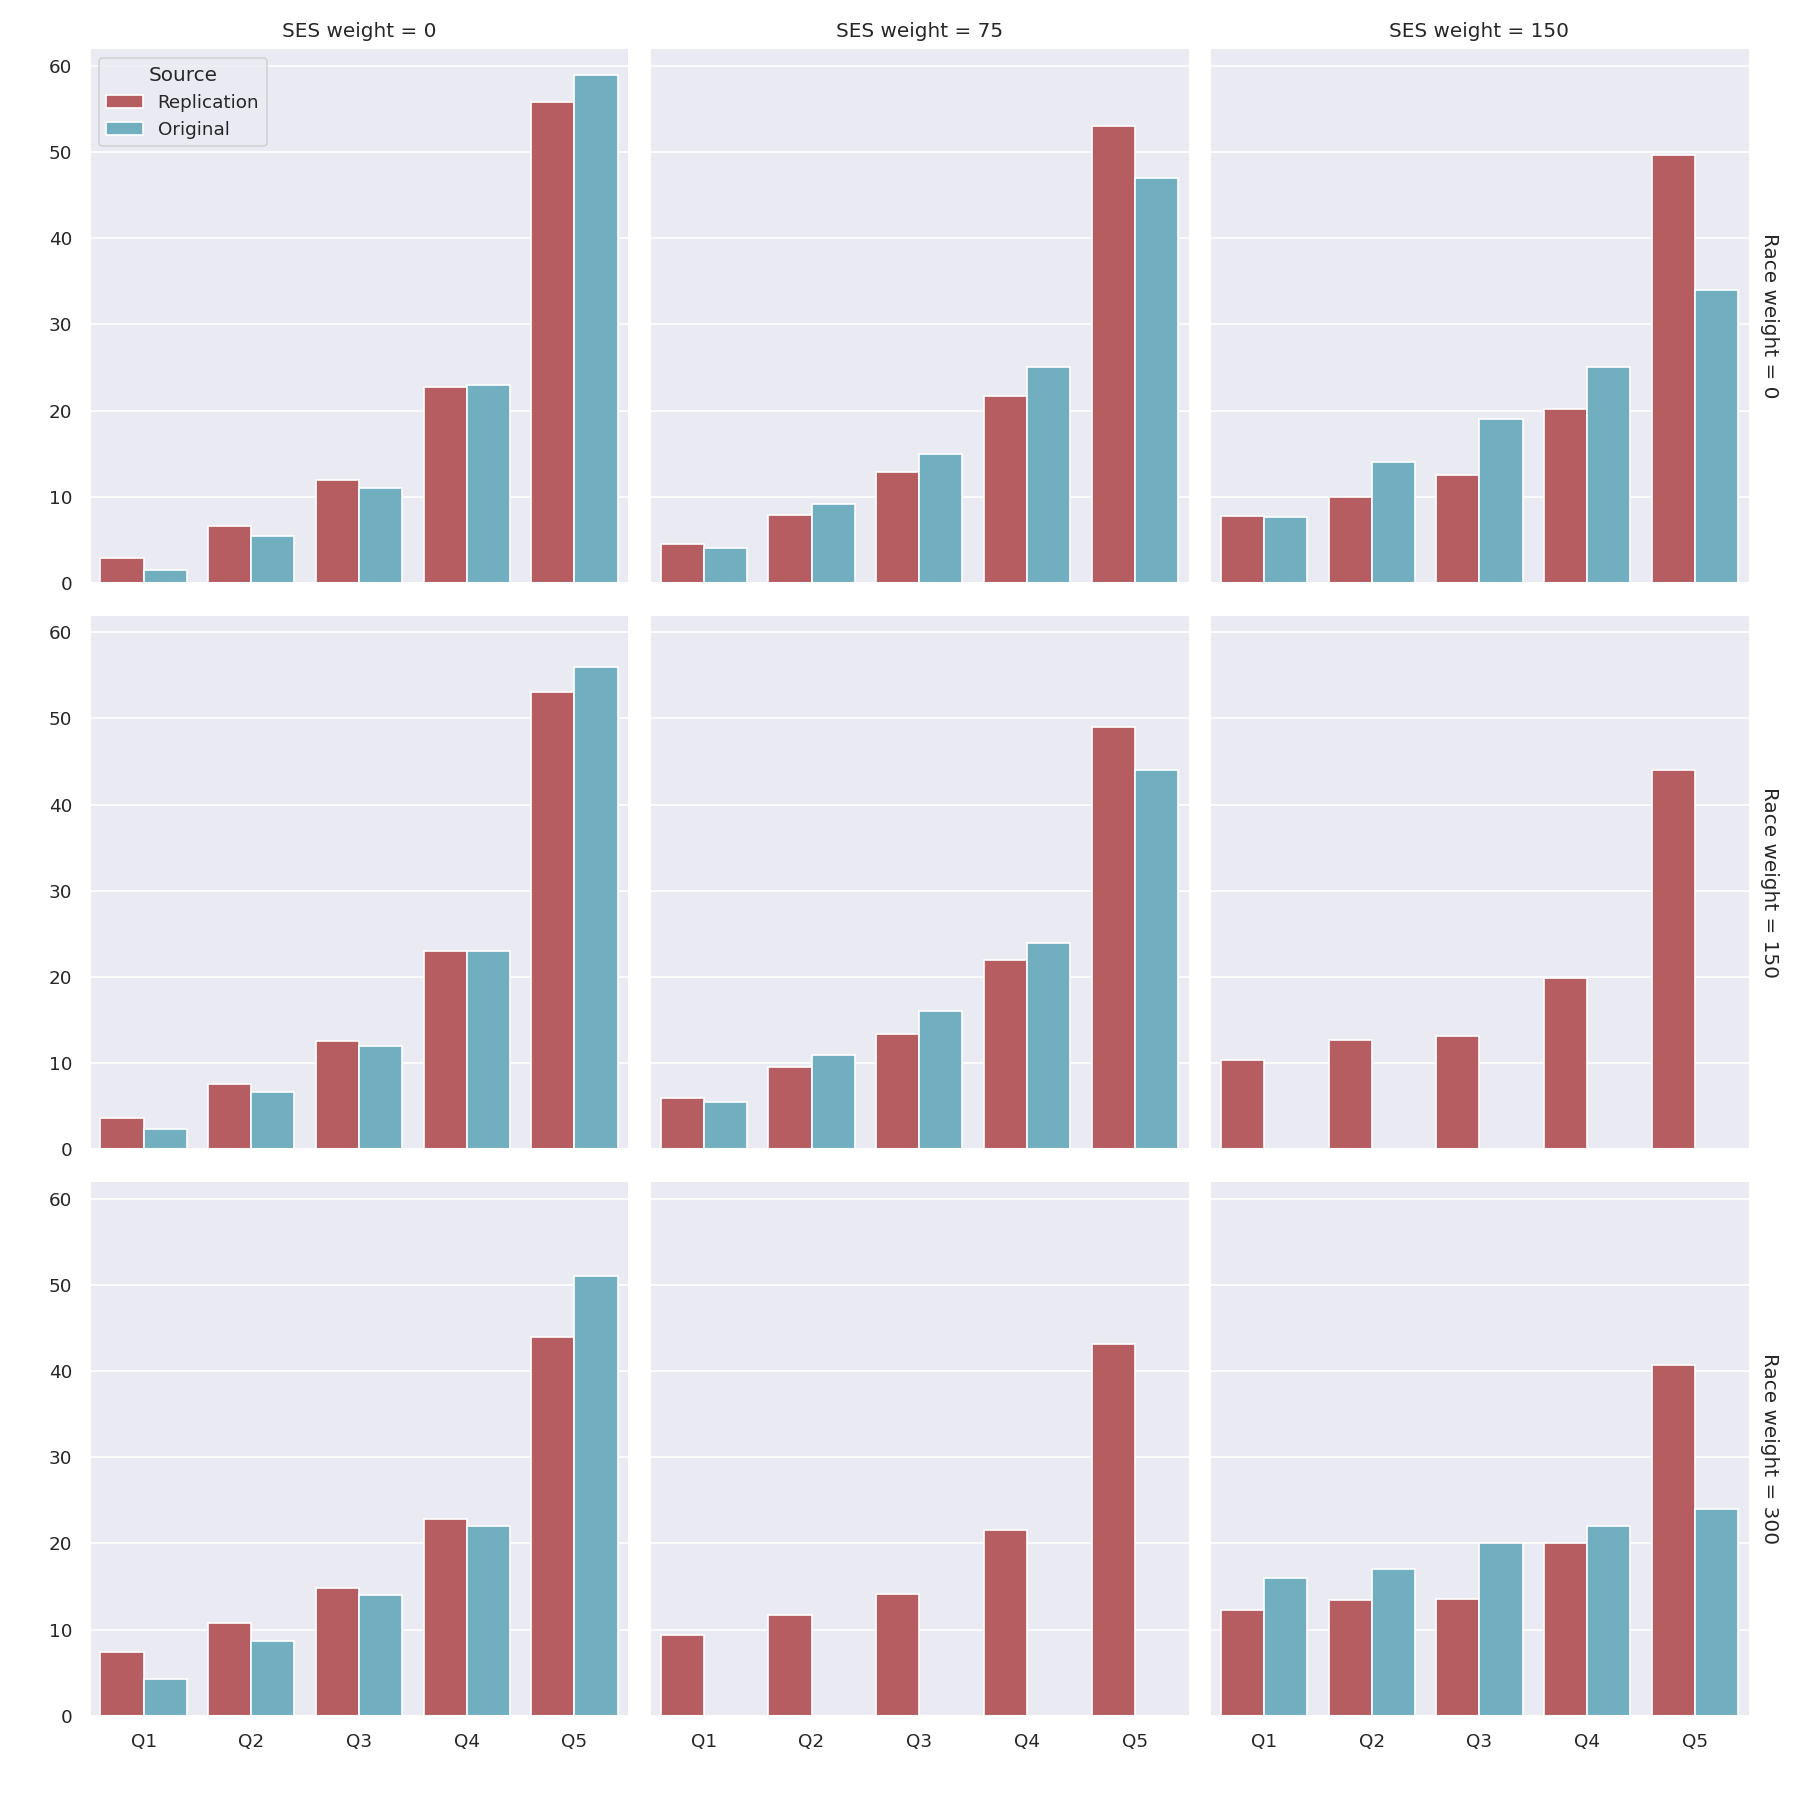
\includegraphics[width=.49\textwidth]{figures/figA5.png}}}
  \caption{Socioeconomic composition of colleges using SES-based and
    racial affirmative actions, by affirmative action weights.}
  \label{fig:A5}
\end{figure}

\section{Results}\label{sec:results}

Our objective was to replicate the overall tendencies of the model.
We compare below our replicated results to the original results.

\begin{description}

\item[Figure~\ref{fig:c1}: success.] The results without using positive discrimination policy presented on Figure~\ref{fig:c1} are similar to the original paper.
The first years appear to exhibit a reversed trend. This could be due to difference in the way the logistic regression is being fitted.

\item[Figure~\ref{fig:c2}: partial success.] Figure~\ref{fig:c2} shows that we replicated the main trends but still indicates an issue with race-based affirmative action: our replication leads to a greater impact on minority students.

\item [Figure~\ref{fig:c4}: partial success.] Looking at Figure~\ref{fig:c4}, the combination of SES-based affirmative action and race-based recruitment is satisfactory in terms of range but the average impact on minority students is lower than the original. This is also the case with Figure~\ref{fig:c3} in Appendix~\ref{sec:add} which considers the same parameters.
However, race-based and SES-based affirmative actions use the same mechanism, which leads us to believe that race‐based recruitment is successfully replicated with a potential issue for SES-based affirmative (as with Figure~\ref{fig:c2}).

\item [Figure~\ref{fig:c5}: success.]  The behavior of quality on Figure~\ref{fig:c5} is similar to the original paper, indicating the adequacy of our quality initialization. A strong claim in the original paper is the decline in quality of colleges using policies, which is not as clear in our replication as only two of the four active colleges suffer such decline. This might be attributed to the lower impact of our actions, as highlighted by the other figures.

\item[Figure~\ref{fig:3a}: partial success.]  Figure~\ref{fig:3a} suffers from the same issue of affirmative actions as Figure~\ref{fig:c2}, but the general behavior is similar to the paper. Figures~\ref{fig:d2} and~\ref{fig:d3} in Appendix~\ref{sec:add} present the same plot for minority and low-income students with varying number of active colleges.

It is important to note that this figure corresponds to an average over 10 runs (as the original paper), which requires the colleges to be sorted by quality. 

The additional left-most arrow covers students who do not enroll. It is unspecified however whether it captures students who do not enroll while having applied, being admitted or without condition. We use the latter (see Appendix~\ref{sec:unenroll}).

\item[Figure~\ref{fig:2}: partial success.]  Figure~\ref{fig:2} shows a successful replication of the general tendency of the model (\emph{i.e.}, the relative values) and a failure in replicating the absolute numbers, probably due to the issue related to the affirmative action observed above.

\item[Figures~\ref{fig:A2} and~\ref{fig:A3}: partial success.] Figures~\ref{fig:A2} and~\ref{fig:A3} shows a successful replication regarding the racial impact of targeted recruiting and SES-based affirmative action strategies, but highlight an issue with the socioeconomic composition (Figure~\ref{fig:A3}). Indeed the impact of our SES-based affirmative action is higher than the original paper.

\item[Figures~\ref{fig:A4} and~\ref{fig:A5}: partial success.] Figures~\ref{fig:A4} and~\ref{fig:A5} lead to the same observation that SES-based affirmative action is not behaving as the original paper. However race-based affirmative action is satisfactory. Note that the combinations (race weight = 150, SES weight = 150) and (race weight = 300, SES weight = 75) are not presented in the original paper.

\end{description}

\section{Conclusion}

In this paper, we presented our attempt at replicating the model presented by \citeauthor{reardon2018levels}~\cite{reardon2018levels}.
The overall behavior is successfully reproduced, with discrepancies regarding the impact of positive discrimination policies.
We attribute the later to issues with our understanding of the paper, thus highlighting the difficulties of describing and understanding complex systems, and the need for open-access to code.
The resulting implementation, while not producing results entirely faithful to the ones from the original paper, can still be useful to simulate data grounded in real-world in the context of college admission.
An extension of this work might consider studying other policies and their interactions, for example with change in policy over time.
We believe however that more efforts are required for this replication to be completely successful--particularly on identifying the sources of the discrepancies--however we hope that this goes towards bridging the gap between computer science and social sciences.

\clearpage

\begin{appendices}

\section{SES-based affirmative action with alternative assumptions}

\begin{figure}[H]
  \centering
  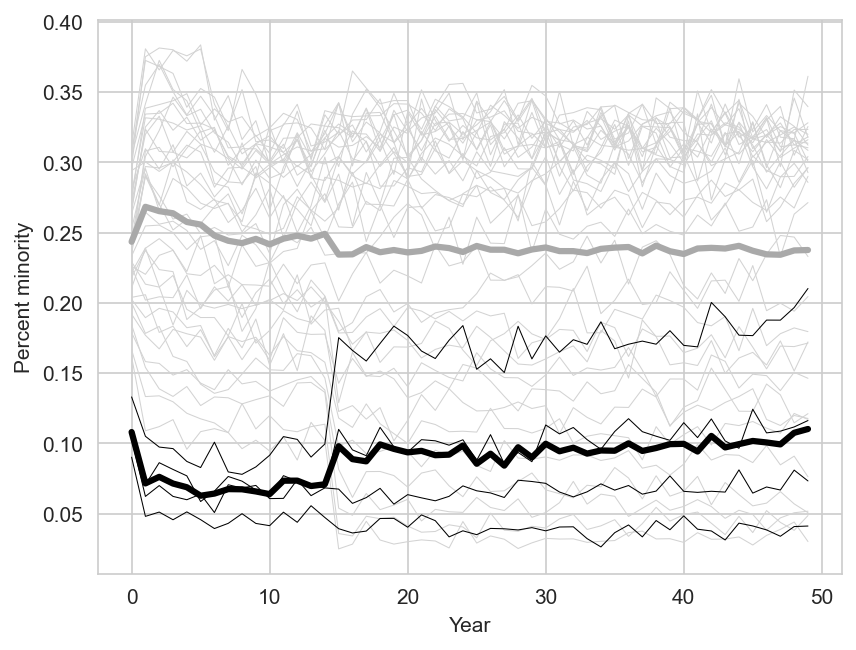
\includegraphics[width=.79\textwidth]{figures/figC4_f1.png}
  \caption{Minority enrollment with the top four colleges using strong SES-based affirmative action (weight of 150) and strong race-based recruitment (weight of 100) \emph{using the formula provided in~\cite{reardon2018levels} for the SES-based affirmative action}. See Section~\ref{sec:diff}}
  \label{fig:c4_f1}
\end{figure}

\begin{figure}[H]
  \centering
  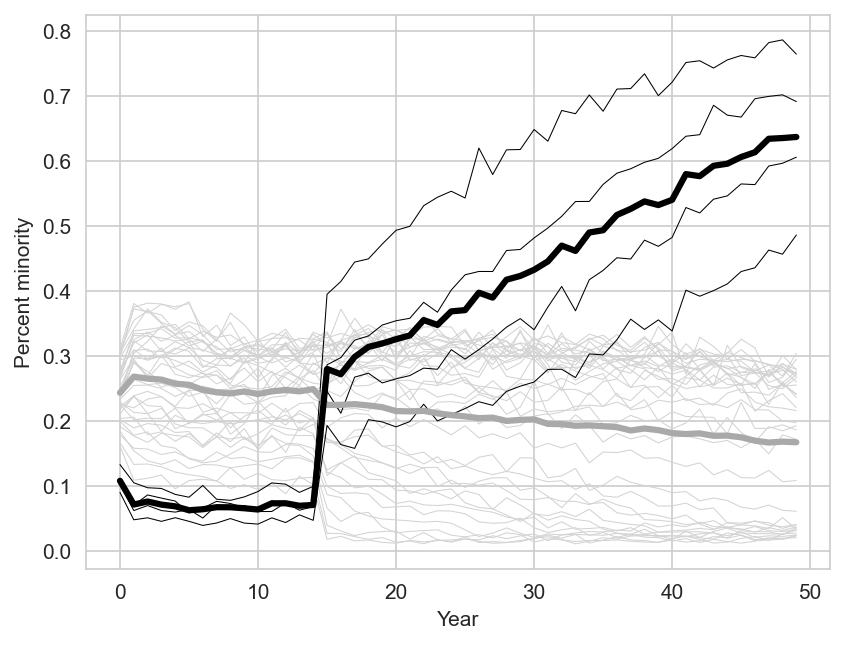
\includegraphics[width=.79\textwidth]{figures/figC4_pen.png}
  \caption{Minority enrollment with the top four colleges using strong SES-based affirmative action (weight of 150) and strong race-based recruitment (weight of 100) \emph{with penalization of high-income students (no truncation to $\geq 0$)}. See Section~\ref{sec:diff}}
  \label{fig:c4_pen}
\end{figure}

\begin{figure}[H]
  \centering
  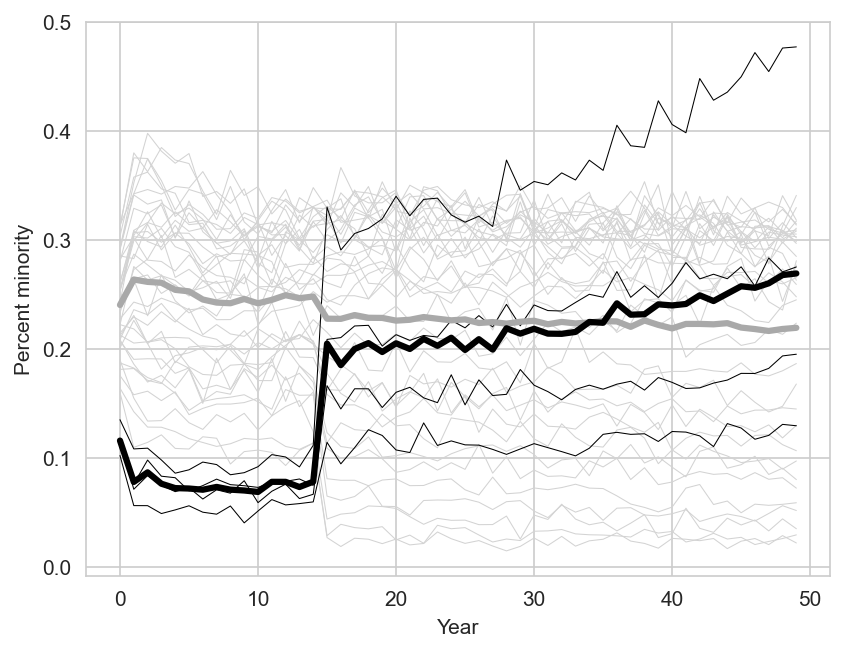
\includegraphics[width=.79\textwidth]{figures/figC4_pq07.png}
  \caption{Minority enrollment with the top four colleges using strong SES-based affirmative action (weight of 150) and strong race-based recruitment (weight of 100) \emph{truncating reliability of student perceptions of college quality to 0.7}. See Section~\ref{sec:diff}}
  \label{fig:c4_pq07}
\end{figure}

\section{Additional figures}\label{sec:add}

\begin{figure}[H]
  \centering
  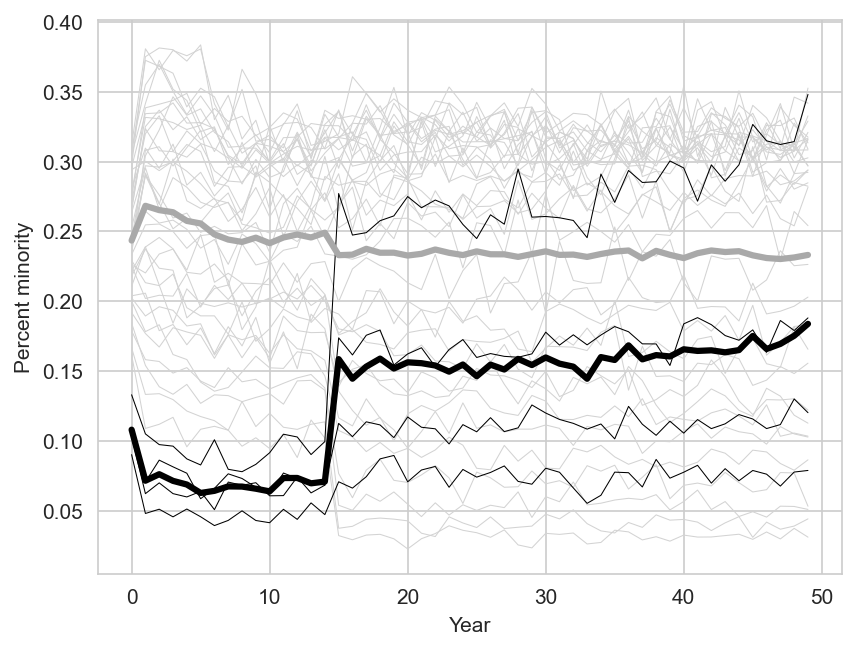
\includegraphics[width=.79\textwidth]{figures/figC3.png}
  \caption{\textquote[{\cite[Figure~C3]{reardon2018levels_preprint}}]{Changes in Black and Hispanic Enrollment over Time with Top 4 Colleges using Moderate SES-Based Affirmative Action and Moderate Race-Based Recruiting}}
  \label{fig:c3}
\end{figure}

\begin{figure}[H]
  \centering
  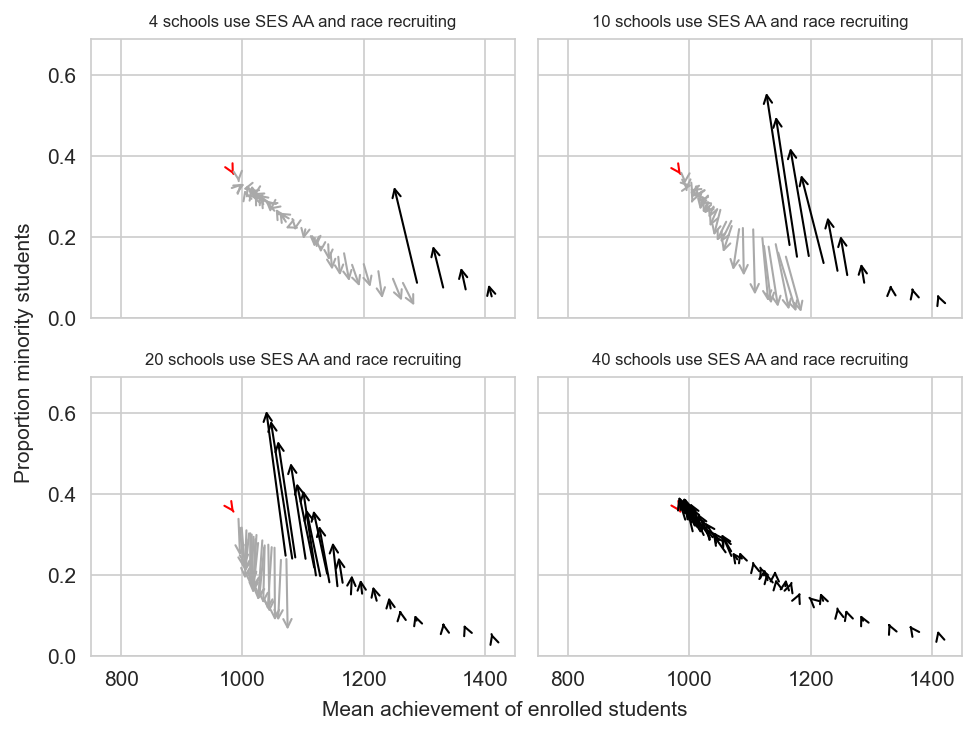
\includegraphics[width=.89\textwidth]{figures/figD2.png}
  \caption{\textquote[{\cite[Figure~D2]{reardon2018levels_preprint}}]{The mean achievement and proportion minority by number of schools using admissions policies.}}
  \label{fig:d2}
\end{figure}

\begin{figure}[H]
  \centering
  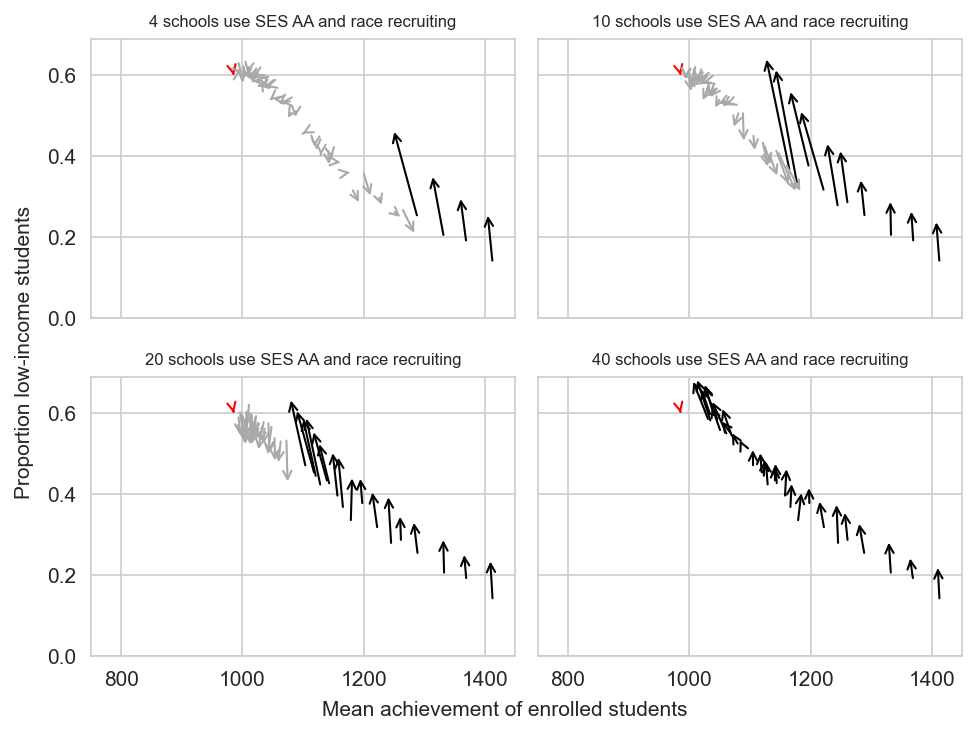
\includegraphics[width=.89\textwidth]{figures/figD3.png}
  \caption{\textquote[{\cite[Figure~D3]{reardon2018levels_preprint}}]{The mean achievement and proportion low-income by number of schools using affirmative
action.}}
  \label{fig:d3}
\end{figure}

\section{Conditional un-enrollment}\label{sec:unenroll}

\begin{table}[H]
    \centering
    \begin{tabular}{l c c c} \toprule
      \textbf{Condition} & \textbf{Mean achievement} & \textbf{Prop. minority students} & \textbf{Prop. low-income students} \\ \midrule
      None               & 990.01                    & 0.35                             & 0.60                               \\
      Applied            & 979.33                    & 0.36                             & 0.59                               \\
      Admitted           & 1177.59                   & 0.17                             & 0.40                               \\ \midrule
      \textbf{Original}  & $\sim 800$                & $\sim 0.6$                       & $\sim 0.5$                         \\ \bottomrule
    \end{tabular}
    \caption{Values for Figure~\ref{fig:3a} (red arrow only) when considering students who do not enroll without condition, while having applied, or while being admitted. The last row displays the values from the original figures.
      Restricting to student having applied gives similar results as having no condition, while capturing only students with an admission gives values further to the original ones.}
    \label{tab:unenroll}
\end{table}


\end{appendices}

\clearpage